%include part: see main.beamer.tex and main.article.tex
\mode<article>{\usepackage{fullpage}}
\mode<presentation>{
    \usetheme{Madrid} %, Madrid, CambridgeUS, Malmoe, Singapore, Berlin
    \useoutertheme{shadow}
} 


\usepackage[russian]{babel}
\usepackage[utf8]{inputenc}
\usepackage{graphicx}
\usepackage{verbatim}


\title[Основы \LaTeX]{Издательская система \LaTeX}
\date{Доклад (\today)}
\author[М.~М.~Шихов]{Михаил Шихов \\ \texttt{\underline{kafevm@mail.ru}}}


\begin{document}


%титул и содержание статьи
\mode<article>{\maketitle\tableofcontents}

%титул и содержание презентации
\frame<presentation>{\titlepage}
\begin{frame}<presentation>[allowframebreaks]
\frametitle{Содержание}
\tableofcontents
\end{frame}


\section{История}

История о создании \TeX ради <<Искусства программирования>>. Используется в википедии, в doxygen.

\begin{frame}
\frametitle{История}
\begin{enumerate}
    \item 1978:\TeX. Дональд Кнут.
    \item 1980-е:\LaTeX. Лесли Лампорт. Разрабатывает надстройку над системой базовых команд \TeX\ с целью более четкого отделения формы от содержания.
    \item 1990-е:\LaTeXe. Дональд Кнут <<замораживает>> \TeX\ и раскрывает исходные коды. Франк Миттельбах, Крис Роули и Райнер Шопф объявили о начале работы над \LaTeX3. Промежуточный результат \LaTeXe\ используется до сих пор.
\end{enumerate}

Из книг по \LaTeXe\ можно рекомендовать \cite{bib:cotelnikov,bib:baldin}. Про \TeX\ от автора \cite{bib:knuthAllAbout}. О типографии в изложении Дональда Кнута \cite{bib:knuthTypograph}.
\end{frame}


\section{Концепции \LaTeX}


\subsection{Содержание и форма}


В каждой предметной области можно выделить подобные разделения содержания и формы. В программировании, например, это паттерн MVC (Model View Controller). Логическая разметка


\begin{frame}
\frametitle{Содержание и форма}
    \begin{columns}
        \column{.48\textwidth}
            \begin{block}{Автор}
                \begin{itemize}
                    \item Новые мысли и идеи.
                    \item Стройность изложения.
                    \item Четкость определений.
                    \item Ясная сюжетная линия.
                    \item Оригинальные примеры, иллюстрации, формулы и таблицы.
                    \item Структура (части, главы, разделы,\ldots).
                    \item Цитирование и ссылки.
                \end{itemize}
            \end{block}
        
        \column{.48\textwidth}
            \begin{block}{Оформитель (издатель)}
                \begin{itemize}
                    \item Гармония восприятия.
                    \item Шрифты, ширина полей, высота отступов\ldots
                    \item Нумерация страниц, разделов, формул\ldots
                    \item Оглавление, предметный указатель\ldots
                    \item Соответствие оформления стандартам (например, ЕСКД).
                \end{itemize}
            \end{block}
    \end{columns}
\end{frame}


\begin{frame}
\frametitle{Исходный \alert{текст}}
    \begin{itemize}
        \item Для обработки текста ничего удобнее текстового редактора\footnote{С подсветкой синтаксиса, подсказками, проверкой правописания.} нет.
        \mode<article> {WYSWYG становится неудобен при больших объемах}
        
        \item Возможность разбить документ на несколько текстовых файлов.
        
        \item Возможность использовать всю мощь систем контроля версий\footnote{Особенно при совместной работе}.
        \mode<article> {Продемонстрировать репозиторий}
        
        \item Возможность работы в <<экстремальных>> условиях\footnote{Текстовый редактор --- это все что нужно автору}.
        
        \item Поддержка комментариев.
        
        \item Простота конструкций логической разметки.
        
        \item Содержание от представления достаточно четко отделено.
        
        \item Выполнение программ на этапе компиляции исходного текста.
        
        \item Возможность определить собственные команды.
        
    \end{itemize}
\end{frame}

\begin{frame}
    \frametitle{\LaTeX-документ в системе контроля версий}
    \framesubtitle{История, ветки, совместная работа\ldots}
    
    \begin{center}
        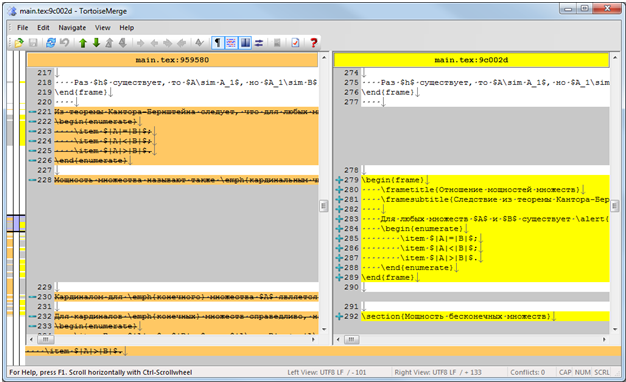
\includegraphics[width=0.8\textwidth]{pict/git}
    \end{center}
\end{frame}


\begin{frame}
\frametitle{Инструменты}
Издательские системы \LaTeX\ (компилятор, утилиты).
\begin{itemize}
    \item Windows
    \begin{itemize}
        \item MiK\TeX.
        \item \TeX\ Live.
    \end{itemize}
    \item Linux
    \begin{itemize}
        \item \TeX\ Live.
    \end{itemize}
    \item Mac
    \begin{itemize}
        \item Mac\TeX.
    \end{itemize}
\end{itemize}
Удобные редакторы исходных текстов: 
\begin{itemize}
    \item IDE Eclipse с плагином \TeX lipse.
    \item Редактор Emacs.
\end{itemize}
\end{frame}


\begin{frame}[fragile]
\frametitle{Класс}

\begin{center}
\verb"\documentclass[<настройки>]{<класс>}"
\end{center}

То, как будет \alert{оформлен} документ определяется его \alert{классом}. Существует множество классов, позволяющие создавать:
\begin{itemize}
    \item Статьи и сборники.
    \item Диссертации.
    \item Книги.
    \item Резюме.
    \item Презентации.
    \item Документы, следующие стандартам\footnote{Дипломы в соответствии с ЕСКД, заявления, стандартные формы}.
    \item и т.д.
\end{itemize}
\end{frame}


\begin{frame}[fragile]
\frametitle{Пакет}

\begin{center}
\verb"\usepackage[<настройки>]{<пакет>}"
\end{center}

Дополнительные \alert{возможности}\footnote{В виде дополнительных конструкций} поставляются в \alert{пакетах}. Существует множество пакетов, позволяющие:
\begin{itemize}
    \item Поддерживать различные кодировки исходного текста.
    \item Вставлять гиперссылки.
    \item Описывать таблицы, вставлять изображения, улучшать формулы.
    \item Писать стихи, пьесы, музыку и песни.
    \item Описывать электронные схемы.
    \item Описывать алгоритмы в псевдокоде.
    \item и т.д.
\end{itemize}
\end{frame}

Поиск пакетов с классами можно произвести на одном из архивов CTAN:


\subsection{CTAN}


\begin{frame}
\frametitle{CTAN}
\begin{definition}
    \alert{CTAN} (Comprehensive \TeX\ Archive Network) --- всеобъемлющая сеть архивов \TeX. Содержит архив классов, пакетов\footnote{Естественно, классы и пакеты хорошо документироаны в формате \TeX}, прикладных программ\footnote{Например, MiK\TeX\ может устанавливать необходимые для компиляции классы и пакеты из CTAN <<на лету>>}.
\end{definition}

Главный сайт \url{http://www.ctan.org/}\\
Огромное количество зеркал по всему миру.\\
Редиректор: \url{http://mirror.ctan.org/}.
\end{frame}

После установки можно найти классы и документацию на них в каталогах на собственном компьютере (показать). Так как \TeX --- это основной инструмент \TeX нического писателя, то вся документация представлена именно в формате \TeX.


\subsection{Компиляция}


Удельный вес информации об отображении в исходном тексте ничтожен --- он насыщен содержанием.


\begin{frame}[fragile]
\frametitle{Компиляция}
Исходный текст \LaTeX размещается в одном или нескольких файлах с расширением *.tex. Чтобы получить красиво \alert{оформленный} документ\footnote{Например, файл <<main.article.tex>> статьи этой презентации} требуется скомпилировать главный файл\footnote{Порядок вызова может быть и другим, например, если требуется построение библиографии программой bibtex}:

\begin{verbatim}
latex main.article.tex
latex main.article.tex
\end{verbatim}
Вы получите *.\alert{dvi} (\alert{d}e\alert{v}ice \alert{i}ndependent) файл документа.

Чтобы получить PDF версию используйте pdflatex:
\begin{verbatim}
pdflatex main.article.tex
pdflatex main.article.tex
\end{verbatim}
\end{frame}


Запуск происходит дважды, потому, что при первом запуске еще не сформирован *.aux файл с данными ссылок. Запуск может выглядеть и по-другому, например, если требуется построение библиографии программой bibtex.

\begin{frame}[fragile]
\frametitle{Компиляция}
\framesubtitle{Служебные файлы}
\begin{itemize}
    \item *.aux --- информация для перекрестного цитирования
    \item *.toc --- оглавление (\verb"\tableofcontents")
    \item *.lof --- список рисунков (\verb"\listoffigures")
    \item *.lot --- список таблиц (\verb"\listoftables")
    \item *.log --- лог
    \item \ldots
\end{itemize}
\end{frame}


\section{Синтаксис}


\subsection{Структура документа и секционирование}

\begin{frame}[fragile,allowframebreaks]
\frametitle{Структура исходного текста \LaTeX}
\begin{verbatim}
\documentclass{article} %указываем класс

%подключаем необходимые пакеты
\usepackage[utf8]{inputenc} %кодировка текста
\usepackage[russian]{babel} %поддержка русского языка
\usepackage{indentfirst} %у русских принято делать 
                         %отступ у первого абзаца

%глобальная настройка командами
\title{Структура \LaTeX\ документа} %название
\author{М.~М.~Шихов} %автор
\date{\today} %дата создания документа

\begin{document} %начало тела документа
    \maketitle %титульный лист
    \begin{abstract}Текст  аннотации.\end{abstract}
    \tableofcontents %оглавление,содержание
    \section{Заглавие первой секции}
    Текст первой секции, абзац первый.

    Текст первой секции, абзац второй.
    \subsection{Заглавие первой подсекции}
    Текст первой подсекции.
\end{document} %конец документа
\end{verbatim}
\end{frame}


\begin{frame}[fragile,allowframebreaks]
\frametitle{Команды, декларации, процедуры}
\begin{itemize}
\item \verb"{<body>}" --- область видимости.
\item \verb"\command[<settings>]{<arguments>}" --- команда.
    \begin{columns}
        \column{.48\textwidth}
            \begin{block}{Содержание}
                \verb"\emph{Логическое} ударение."\\
                \verb"Замечание\footnote{Примечание}"
            \end{block}
        
        \column{.48\textwidth}
            \begin{block}{Форма}
                \emph{Логическое} ударение.
                Замечание\footnote{Примечание}
            \end{block}
    \end{columns}

\item \verb"{\declaration[<settings>]}" --- декларация.
    \begin{columns}
        \column{.48\textwidth}
            \begin{block}{Содержание}
                \verb"{\em Логическое} ударение."\\
                \verb"{\bf Жирный} текст"
            \end{block}
        
        \column{.48\textwidth}
            \begin{block}{Форма}
                {\em Логическое} ударение.
                {\bf Жирный} текст
            \end{block}
    \end{columns}
    
\item \verb"\begin{command}[<settings>]<body>\end{command}" --- процедура.
    \begin{columns}
        \column{.48\textwidth}
            \begin{block}{Содержание}
                \begin{verbatim}
\begin{enumerate}                
    \item Раз элемент 
    \item Два элемент 
\end{enumerate}                
                \end{verbatim}
            \end{block}
        
        \column{.48\textwidth}
            \begin{block}{Форма}
                \begin{enumerate}                
                    \item Раз элемент 
                    \item Два элемент 
                \end{enumerate}                
            \end{block}
    \end{columns}

\end{itemize}
\begin{verbatim}
\end{verbatim}
\end{frame}


\begin{frame}[fragile,allowframebreaks]
    \frametitle{Собственные команды}

    \newcommand{\MyBinaryAdditionTask}[3]{
      Ссмложить целые числа A={#1} и B={#2} в \emph{двоичной} 
      системе счисления, в {#3}, в 8 разрядной сетке, 
      где 7-й разряд является знаковым.
    }
    
Например, перед телом документа объявим собственную команду:
\begin{semiverbatim}  
\\newcommand\{\alert{\\MyBinaryAdditionTask}\}[\alert{3}]\{
  С\alert{см}ложить целые числа A=\{\alert{\#1}\} и B=\{\alert{\#2}\} в \\emph\{двоичной\} 
  системе счисления, в \{\alert{\#3}\}, в 8 разрядной сетке, где 7-й 
  разряд является знаковым.
\}  
\end{semiverbatim}    

И используем много раз в тексте\footnote{Опечатку <<Ссмложить>> нужно исправить в \alert{одном} месте}:
\begin{semiverbatim}  
\\begin\{enumerate\}
    \\item \\MyBinaryAdditionTask\{10\}\{20\}\{ОК\}
    \\item \\MyBinaryAdditionTask\{20\}\{30\}\{ДК\}
    \\item \\MyBinaryAdditionTask\{30\}\{40\}\{ПК\}
    \\item \ldots
\\end\{enumerate\}
\end{semiverbatim}    

Получив следующий результат:
\begin{enumerate}
    \item \MyBinaryAdditionTask{10}{20}{ОК}
    \item \MyBinaryAdditionTask{20}{30}{ДК}
    \item \MyBinaryAdditionTask{30}{40}{ПК}
    \item \ldots
\end{enumerate}

\end{frame}


\begin{frame}[fragile]
\frametitle{Включения файлов}
Иногда бывает удобно разбить исходный текст на несколько частей, например по \alert{главам}, или выделить \alert{общие части} двух печатных документов. Это можно сделать с помощью команды
\begin{verbatim}
\input{<относительный путь к файлу>}
%расширение *.tex в имени файла указывать не надо
\end{verbatim}
Например, главный файл презентации main.beamer.tex так включает общую часть main.tex:
\begin{verbatim}
\documentclass[ignorenonframetext,red,utf8]{beamer}
%include part: see main.beamer.tex and main.article.tex
\mode<article>{\usepackage{fullpage}}
\mode<presentation>{
    \usetheme{Madrid} %, Madrid, CambridgeUS, Malmoe, Singapore, Berlin
    \useoutertheme{shadow}
} 


\usepackage[russian]{babel}
\usepackage[utf8]{inputenc}
\usepackage{graphicx}
\usepackage{verbatim}


\title[Основы \LaTeX]{Издательская система \LaTeX}
\date{Доклад (\today)}
\author[М.~М.~Шихов]{Михаил Шихов \\ \texttt{\underline{kafevm@mail.ru}}}


\begin{document}


%титул и содержание статьи
\mode<article>{\maketitle\tableofcontents}

%титул и содержание презентации
\frame<presentation>{\titlepage}
\begin{frame}<presentation>[allowframebreaks]
\frametitle{Содержание}
\tableofcontents
\end{frame}


\section{История}

История о создании \TeX ради <<Искусства программирования>>. Используется в википедии, в doxygen.

\begin{frame}
\frametitle{История}
\begin{enumerate}
    \item 1978:\TeX. Дональд Кнут.
    \item 1980-е:\LaTeX. Лесли Лампорт. Разрабатывает надстройку над системой базовых команд \TeX\ с целью более четкого отделения формы от содержания.
    \item 1990-е:\LaTeXe. Дональд Кнут <<замораживает>> \TeX\ и раскрывает исходные коды. Франк Миттельбах, Крис Роули и Райнер Шопф объявили о начале работы над \LaTeX3. Промежуточный результат \LaTeXe\ используется до сих пор.
\end{enumerate}

Из книг по \LaTeXe\ можно рекомендовать \cite{bib:cotelnikov,bib:baldin}. Про \TeX\ от автора \cite{bib:knuthAllAbout}. О типографии в изложении Дональда Кнута \cite{bib:knuthTypograph}.
\end{frame}


\section{Концепции \LaTeX}


\subsection{Содержание и форма}


В каждой предметной области можно выделить подобные разделения содержания и формы. В программировании, например, это паттерн MVC (Model View Controller). Логическая разметка


\begin{frame}
\frametitle{Содержание и форма}
    \begin{columns}
        \column{.48\textwidth}
            \begin{block}{Автор}
                \begin{itemize}
                    \item Новые мысли и идеи.
                    \item Стройность изложения.
                    \item Четкость определений.
                    \item Ясная сюжетная линия.
                    \item Оригинальные примеры, иллюстрации, формулы и таблицы.
                    \item Структура (части, главы, разделы,\ldots).
                    \item Цитирование и ссылки.
                \end{itemize}
            \end{block}
        
        \column{.48\textwidth}
            \begin{block}{Оформитель (издатель)}
                \begin{itemize}
                    \item Гармония восприятия.
                    \item Шрифты, ширина полей, высота отступов\ldots
                    \item Нумерация страниц, разделов, формул\ldots
                    \item Оглавление, предметный указатель\ldots
                    \item Соответствие оформления стандартам (например, ЕСКД).
                \end{itemize}
            \end{block}
    \end{columns}
\end{frame}


\begin{frame}
\frametitle{Исходный \alert{текст}}
    \begin{itemize}
        \item Для обработки текста ничего удобнее текстового редактора\footnote{С подсветкой синтаксиса, подсказками, проверкой правописания.} нет.
        \mode<article> {WYSWYG становится неудобен при больших объемах}
        
        \item Возможность разбить документ на несколько текстовых файлов.
        
        \item Возможность использовать всю мощь систем контроля версий\footnote{Особенно при совместной работе}.
        \mode<article> {Продемонстрировать репозиторий}
        
        \item Возможность работы в <<экстремальных>> условиях\footnote{Текстовый редактор --- это все что нужно автору}.
        
        \item Поддержка комментариев.
        
        \item Простота конструкций логической разметки.
        
        \item Содержание от представления достаточно четко отделено.
        
        \item Выполнение программ на этапе компиляции исходного текста.
        
        \item Возможность определить собственные команды.
        
    \end{itemize}
\end{frame}

\begin{frame}
    \frametitle{\LaTeX-документ в системе контроля версий}
    \framesubtitle{История, ветки, совместная работа\ldots}
    
    \begin{center}
        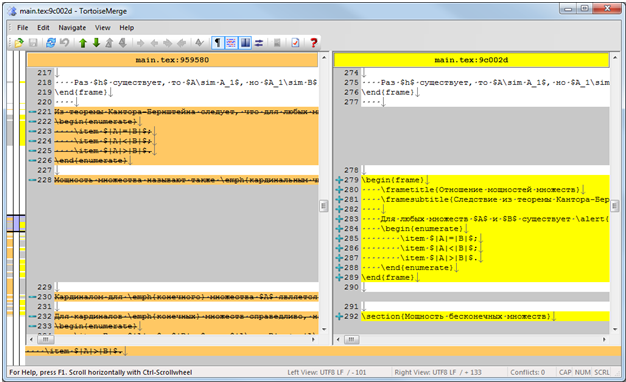
\includegraphics[width=0.8\textwidth]{pict/git}
    \end{center}
\end{frame}


\begin{frame}
\frametitle{Инструменты}
Издательские системы \LaTeX\ (компилятор, утилиты).
\begin{itemize}
    \item Windows
    \begin{itemize}
        \item MiK\TeX.
        \item \TeX\ Live.
    \end{itemize}
    \item Linux
    \begin{itemize}
        \item \TeX\ Live.
    \end{itemize}
    \item Mac
    \begin{itemize}
        \item Mac\TeX.
    \end{itemize}
\end{itemize}
Удобные редакторы исходных текстов: 
\begin{itemize}
    \item IDE Eclipse с плагином \TeX lipse.
    \item Редактор Emacs.
\end{itemize}
\end{frame}


\begin{frame}[fragile]
\frametitle{Класс}

\begin{center}
\verb"\documentclass[<настройки>]{<класс>}"
\end{center}

То, как будет \alert{оформлен} документ определяется его \alert{классом}. Существует множество классов, позволяющие создавать:
\begin{itemize}
    \item Статьи и сборники.
    \item Диссертации.
    \item Книги.
    \item Резюме.
    \item Презентации.
    \item Документы, следующие стандартам\footnote{Дипломы в соответствии с ЕСКД, заявления, стандартные формы}.
    \item и т.д.
\end{itemize}
\end{frame}


\begin{frame}[fragile]
\frametitle{Пакет}

\begin{center}
\verb"\usepackage[<настройки>]{<пакет>}"
\end{center}

Дополнительные \alert{возможности}\footnote{В виде дополнительных конструкций} поставляются в \alert{пакетах}. Существует множество пакетов, позволяющие:
\begin{itemize}
    \item Поддерживать различные кодировки исходного текста.
    \item Вставлять гиперссылки.
    \item Описывать таблицы, вставлять изображения, улучшать формулы.
    \item Писать стихи, пьесы, музыку и песни.
    \item Описывать электронные схемы.
    \item Описывать алгоритмы в псевдокоде.
    \item и т.д.
\end{itemize}
\end{frame}

Поиск пакетов с классами можно произвести на одном из архивов CTAN:


\subsection{CTAN}


\begin{frame}
\frametitle{CTAN}
\begin{definition}
    \alert{CTAN} (Comprehensive \TeX\ Archive Network) --- всеобъемлющая сеть архивов \TeX. Содержит архив классов, пакетов\footnote{Естественно, классы и пакеты хорошо документироаны в формате \TeX}, прикладных программ\footnote{Например, MiK\TeX\ может устанавливать необходимые для компиляции классы и пакеты из CTAN <<на лету>>}.
\end{definition}

Главный сайт \url{http://www.ctan.org/}\\
Огромное количество зеркал по всему миру.\\
Редиректор: \url{http://mirror.ctan.org/}.
\end{frame}

После установки можно найти классы и документацию на них в каталогах на собственном компьютере (показать). Так как \TeX --- это основной инструмент \TeX нического писателя, то вся документация представлена именно в формате \TeX.


\subsection{Компиляция}


Удельный вес информации об отображении в исходном тексте ничтожен --- он насыщен содержанием.


\begin{frame}[fragile]
\frametitle{Компиляция}
Исходный текст \LaTeX размещается в одном или нескольких файлах с расширением *.tex. Чтобы получить красиво \alert{оформленный} документ\footnote{Например, файл <<main.article.tex>> статьи этой презентации} требуется скомпилировать главный файл\footnote{Порядок вызова может быть и другим, например, если требуется построение библиографии программой bibtex}:

\begin{verbatim}
latex main.article.tex
latex main.article.tex
\end{verbatim}
Вы получите *.\alert{dvi} (\alert{d}e\alert{v}ice \alert{i}ndependent) файл документа.

Чтобы получить PDF версию используйте pdflatex:
\begin{verbatim}
pdflatex main.article.tex
pdflatex main.article.tex
\end{verbatim}
\end{frame}


Запуск происходит дважды, потому, что при первом запуске еще не сформирован *.aux файл с данными ссылок. Запуск может выглядеть и по-другому, например, если требуется построение библиографии программой bibtex.

\begin{frame}[fragile]
\frametitle{Компиляция}
\framesubtitle{Служебные файлы}
\begin{itemize}
    \item *.aux --- информация для перекрестного цитирования
    \item *.toc --- оглавление (\verb"\tableofcontents")
    \item *.lof --- список рисунков (\verb"\listoffigures")
    \item *.lot --- список таблиц (\verb"\listoftables")
    \item *.log --- лог
    \item \ldots
\end{itemize}
\end{frame}


\section{Синтаксис}


\subsection{Структура документа и секционирование}

\begin{frame}[fragile,allowframebreaks]
\frametitle{Структура исходного текста \LaTeX}
\begin{verbatim}
\documentclass{article} %указываем класс

%подключаем необходимые пакеты
\usepackage[utf8]{inputenc} %кодировка текста
\usepackage[russian]{babel} %поддержка русского языка
\usepackage{indentfirst} %у русских принято делать 
                         %отступ у первого абзаца

%глобальная настройка командами
\title{Структура \LaTeX\ документа} %название
\author{М.~М.~Шихов} %автор
\date{\today} %дата создания документа

\begin{document} %начало тела документа
    \maketitle %титульный лист
    \begin{abstract}Текст  аннотации.\end{abstract}
    \tableofcontents %оглавление,содержание
    \section{Заглавие первой секции}
    Текст первой секции, абзац первый.

    Текст первой секции, абзац второй.
    \subsection{Заглавие первой подсекции}
    Текст первой подсекции.
\end{document} %конец документа
\end{verbatim}
\end{frame}


\begin{frame}[fragile,allowframebreaks]
\frametitle{Команды, декларации, процедуры}
\begin{itemize}
\item \verb"{<body>}" --- область видимости.
\item \verb"\command[<settings>]{<arguments>}" --- команда.
    \begin{columns}
        \column{.48\textwidth}
            \begin{block}{Содержание}
                \verb"\emph{Логическое} ударение."\\
                \verb"Замечание\footnote{Примечание}"
            \end{block}
        
        \column{.48\textwidth}
            \begin{block}{Форма}
                \emph{Логическое} ударение.
                Замечание\footnote{Примечание}
            \end{block}
    \end{columns}

\item \verb"{\declaration[<settings>]}" --- декларация.
    \begin{columns}
        \column{.48\textwidth}
            \begin{block}{Содержание}
                \verb"{\em Логическое} ударение."\\
                \verb"{\bf Жирный} текст"
            \end{block}
        
        \column{.48\textwidth}
            \begin{block}{Форма}
                {\em Логическое} ударение.
                {\bf Жирный} текст
            \end{block}
    \end{columns}
    
\item \verb"\begin{command}[<settings>]<body>\end{command}" --- процедура.
    \begin{columns}
        \column{.48\textwidth}
            \begin{block}{Содержание}
                \begin{verbatim}
\begin{enumerate}                
    \item Раз элемент 
    \item Два элемент 
\end{enumerate}                
                \end{verbatim}
            \end{block}
        
        \column{.48\textwidth}
            \begin{block}{Форма}
                \begin{enumerate}                
                    \item Раз элемент 
                    \item Два элемент 
                \end{enumerate}                
            \end{block}
    \end{columns}

\end{itemize}
\begin{verbatim}
\end{verbatim}
\end{frame}


\begin{frame}[fragile,allowframebreaks]
    \frametitle{Собственные команды}

    \newcommand{\MyBinaryAdditionTask}[3]{
      Ссмложить целые числа A={#1} и B={#2} в \emph{двоичной} 
      системе счисления, в {#3}, в 8 разрядной сетке, 
      где 7-й разряд является знаковым.
    }
    
Например, перед телом документа объявим собственную команду:
\begin{semiverbatim}  
\\newcommand\{\alert{\\MyBinaryAdditionTask}\}[\alert{3}]\{
  С\alert{см}ложить целые числа A=\{\alert{\#1}\} и B=\{\alert{\#2}\} в \\emph\{двоичной\} 
  системе счисления, в \{\alert{\#3}\}, в 8 разрядной сетке, где 7-й 
  разряд является знаковым.
\}  
\end{semiverbatim}    

И используем много раз в тексте\footnote{Опечатку <<Ссмложить>> нужно исправить в \alert{одном} месте}:
\begin{semiverbatim}  
\\begin\{enumerate\}
    \\item \\MyBinaryAdditionTask\{10\}\{20\}\{ОК\}
    \\item \\MyBinaryAdditionTask\{20\}\{30\}\{ДК\}
    \\item \\MyBinaryAdditionTask\{30\}\{40\}\{ПК\}
    \\item \ldots
\\end\{enumerate\}
\end{semiverbatim}    

Получив следующий результат:
\begin{enumerate}
    \item \MyBinaryAdditionTask{10}{20}{ОК}
    \item \MyBinaryAdditionTask{20}{30}{ДК}
    \item \MyBinaryAdditionTask{30}{40}{ПК}
    \item \ldots
\end{enumerate}

\end{frame}


\begin{frame}[fragile]
\frametitle{Включения файлов}
Иногда бывает удобно разбить исходный текст на несколько частей, например по \alert{главам}, или выделить \alert{общие части} двух печатных документов. Это можно сделать с помощью команды
\begin{verbatim}
\input{<относительный путь к файлу>}
%расширение *.tex в имени файла указывать не надо
\end{verbatim}
Например, главный файл презентации main.beamer.tex так включает общую часть main.tex:
\begin{verbatim}
\documentclass[ignorenonframetext,red,utf8]{beamer}
%include part: see main.beamer.tex and main.article.tex
\mode<article>{\usepackage{fullpage}}
\mode<presentation>{
    \usetheme{Madrid} %, Madrid, CambridgeUS, Malmoe, Singapore, Berlin
    \useoutertheme{shadow}
} 


\usepackage[russian]{babel}
\usepackage[utf8]{inputenc}
\usepackage{graphicx}
\usepackage{verbatim}


\title[Основы \LaTeX]{Издательская система \LaTeX}
\date{Доклад (\today)}
\author[М.~М.~Шихов]{Михаил Шихов \\ \texttt{\underline{kafevm@mail.ru}}}


\begin{document}


%титул и содержание статьи
\mode<article>{\maketitle\tableofcontents}

%титул и содержание презентации
\frame<presentation>{\titlepage}
\begin{frame}<presentation>[allowframebreaks]
\frametitle{Содержание}
\tableofcontents
\end{frame}


\section{История}

История о создании \TeX ради <<Искусства программирования>>. Используется в википедии, в doxygen.

\begin{frame}
\frametitle{История}
\begin{enumerate}
    \item 1978:\TeX. Дональд Кнут.
    \item 1980-е:\LaTeX. Лесли Лампорт. Разрабатывает надстройку над системой базовых команд \TeX\ с целью более четкого отделения формы от содержания.
    \item 1990-е:\LaTeXe. Дональд Кнут <<замораживает>> \TeX\ и раскрывает исходные коды. Франк Миттельбах, Крис Роули и Райнер Шопф объявили о начале работы над \LaTeX3. Промежуточный результат \LaTeXe\ используется до сих пор.
\end{enumerate}

Из книг по \LaTeXe\ можно рекомендовать \cite{bib:cotelnikov,bib:baldin}. Про \TeX\ от автора \cite{bib:knuthAllAbout}. О типографии в изложении Дональда Кнута \cite{bib:knuthTypograph}.
\end{frame}


\section{Концепции \LaTeX}


\subsection{Содержание и форма}


В каждой предметной области можно выделить подобные разделения содержания и формы. В программировании, например, это паттерн MVC (Model View Controller). Логическая разметка


\begin{frame}
\frametitle{Содержание и форма}
    \begin{columns}
        \column{.48\textwidth}
            \begin{block}{Автор}
                \begin{itemize}
                    \item Новые мысли и идеи.
                    \item Стройность изложения.
                    \item Четкость определений.
                    \item Ясная сюжетная линия.
                    \item Оригинальные примеры, иллюстрации, формулы и таблицы.
                    \item Структура (части, главы, разделы,\ldots).
                    \item Цитирование и ссылки.
                \end{itemize}
            \end{block}
        
        \column{.48\textwidth}
            \begin{block}{Оформитель (издатель)}
                \begin{itemize}
                    \item Гармония восприятия.
                    \item Шрифты, ширина полей, высота отступов\ldots
                    \item Нумерация страниц, разделов, формул\ldots
                    \item Оглавление, предметный указатель\ldots
                    \item Соответствие оформления стандартам (например, ЕСКД).
                \end{itemize}
            \end{block}
    \end{columns}
\end{frame}


\begin{frame}
\frametitle{Исходный \alert{текст}}
    \begin{itemize}
        \item Для обработки текста ничего удобнее текстового редактора\footnote{С подсветкой синтаксиса, подсказками, проверкой правописания.} нет.
        \mode<article> {WYSWYG становится неудобен при больших объемах}
        
        \item Возможность разбить документ на несколько текстовых файлов.
        
        \item Возможность использовать всю мощь систем контроля версий\footnote{Особенно при совместной работе}.
        \mode<article> {Продемонстрировать репозиторий}
        
        \item Возможность работы в <<экстремальных>> условиях\footnote{Текстовый редактор --- это все что нужно автору}.
        
        \item Поддержка комментариев.
        
        \item Простота конструкций логической разметки.
        
        \item Содержание от представления достаточно четко отделено.
        
        \item Выполнение программ на этапе компиляции исходного текста.
        
        \item Возможность определить собственные команды.
        
    \end{itemize}
\end{frame}

\begin{frame}
    \frametitle{\LaTeX-документ в системе контроля версий}
    \framesubtitle{История, ветки, совместная работа\ldots}
    
    \begin{center}
        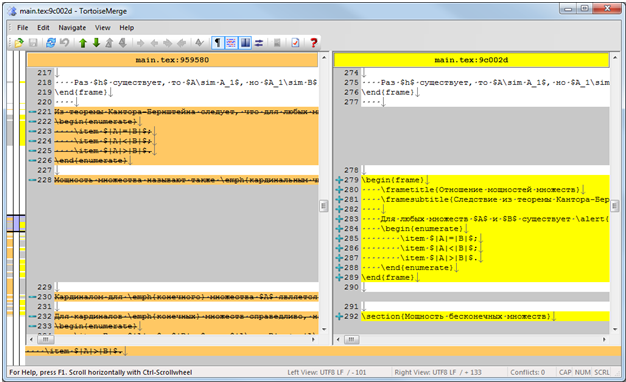
\includegraphics[width=0.8\textwidth]{pict/git}
    \end{center}
\end{frame}


\begin{frame}
\frametitle{Инструменты}
Издательские системы \LaTeX\ (компилятор, утилиты).
\begin{itemize}
    \item Windows
    \begin{itemize}
        \item MiK\TeX.
        \item \TeX\ Live.
    \end{itemize}
    \item Linux
    \begin{itemize}
        \item \TeX\ Live.
    \end{itemize}
    \item Mac
    \begin{itemize}
        \item Mac\TeX.
    \end{itemize}
\end{itemize}
Удобные редакторы исходных текстов: 
\begin{itemize}
    \item IDE Eclipse с плагином \TeX lipse.
    \item Редактор Emacs.
\end{itemize}
\end{frame}


\begin{frame}[fragile]
\frametitle{Класс}

\begin{center}
\verb"\documentclass[<настройки>]{<класс>}"
\end{center}

То, как будет \alert{оформлен} документ определяется его \alert{классом}. Существует множество классов, позволяющие создавать:
\begin{itemize}
    \item Статьи и сборники.
    \item Диссертации.
    \item Книги.
    \item Резюме.
    \item Презентации.
    \item Документы, следующие стандартам\footnote{Дипломы в соответствии с ЕСКД, заявления, стандартные формы}.
    \item и т.д.
\end{itemize}
\end{frame}


\begin{frame}[fragile]
\frametitle{Пакет}

\begin{center}
\verb"\usepackage[<настройки>]{<пакет>}"
\end{center}

Дополнительные \alert{возможности}\footnote{В виде дополнительных конструкций} поставляются в \alert{пакетах}. Существует множество пакетов, позволяющие:
\begin{itemize}
    \item Поддерживать различные кодировки исходного текста.
    \item Вставлять гиперссылки.
    \item Описывать таблицы, вставлять изображения, улучшать формулы.
    \item Писать стихи, пьесы, музыку и песни.
    \item Описывать электронные схемы.
    \item Описывать алгоритмы в псевдокоде.
    \item и т.д.
\end{itemize}
\end{frame}

Поиск пакетов с классами можно произвести на одном из архивов CTAN:


\subsection{CTAN}


\begin{frame}
\frametitle{CTAN}
\begin{definition}
    \alert{CTAN} (Comprehensive \TeX\ Archive Network) --- всеобъемлющая сеть архивов \TeX. Содержит архив классов, пакетов\footnote{Естественно, классы и пакеты хорошо документироаны в формате \TeX}, прикладных программ\footnote{Например, MiK\TeX\ может устанавливать необходимые для компиляции классы и пакеты из CTAN <<на лету>>}.
\end{definition}

Главный сайт \url{http://www.ctan.org/}\\
Огромное количество зеркал по всему миру.\\
Редиректор: \url{http://mirror.ctan.org/}.
\end{frame}

После установки можно найти классы и документацию на них в каталогах на собственном компьютере (показать). Так как \TeX --- это основной инструмент \TeX нического писателя, то вся документация представлена именно в формате \TeX.


\subsection{Компиляция}


Удельный вес информации об отображении в исходном тексте ничтожен --- он насыщен содержанием.


\begin{frame}[fragile]
\frametitle{Компиляция}
Исходный текст \LaTeX размещается в одном или нескольких файлах с расширением *.tex. Чтобы получить красиво \alert{оформленный} документ\footnote{Например, файл <<main.article.tex>> статьи этой презентации} требуется скомпилировать главный файл\footnote{Порядок вызова может быть и другим, например, если требуется построение библиографии программой bibtex}:

\begin{verbatim}
latex main.article.tex
latex main.article.tex
\end{verbatim}
Вы получите *.\alert{dvi} (\alert{d}e\alert{v}ice \alert{i}ndependent) файл документа.

Чтобы получить PDF версию используйте pdflatex:
\begin{verbatim}
pdflatex main.article.tex
pdflatex main.article.tex
\end{verbatim}
\end{frame}


Запуск происходит дважды, потому, что при первом запуске еще не сформирован *.aux файл с данными ссылок. Запуск может выглядеть и по-другому, например, если требуется построение библиографии программой bibtex.

\begin{frame}[fragile]
\frametitle{Компиляция}
\framesubtitle{Служебные файлы}
\begin{itemize}
    \item *.aux --- информация для перекрестного цитирования
    \item *.toc --- оглавление (\verb"\tableofcontents")
    \item *.lof --- список рисунков (\verb"\listoffigures")
    \item *.lot --- список таблиц (\verb"\listoftables")
    \item *.log --- лог
    \item \ldots
\end{itemize}
\end{frame}


\section{Синтаксис}


\subsection{Структура документа и секционирование}

\begin{frame}[fragile,allowframebreaks]
\frametitle{Структура исходного текста \LaTeX}
\begin{verbatim}
\documentclass{article} %указываем класс

%подключаем необходимые пакеты
\usepackage[utf8]{inputenc} %кодировка текста
\usepackage[russian]{babel} %поддержка русского языка
\usepackage{indentfirst} %у русских принято делать 
                         %отступ у первого абзаца

%глобальная настройка командами
\title{Структура \LaTeX\ документа} %название
\author{М.~М.~Шихов} %автор
\date{\today} %дата создания документа

\begin{document} %начало тела документа
    \maketitle %титульный лист
    \begin{abstract}Текст  аннотации.\end{abstract}
    \tableofcontents %оглавление,содержание
    \section{Заглавие первой секции}
    Текст первой секции, абзац первый.

    Текст первой секции, абзац второй.
    \subsection{Заглавие первой подсекции}
    Текст первой подсекции.
\end{document} %конец документа
\end{verbatim}
\end{frame}


\begin{frame}[fragile,allowframebreaks]
\frametitle{Команды, декларации, процедуры}
\begin{itemize}
\item \verb"{<body>}" --- область видимости.
\item \verb"\command[<settings>]{<arguments>}" --- команда.
    \begin{columns}
        \column{.48\textwidth}
            \begin{block}{Содержание}
                \verb"\emph{Логическое} ударение."\\
                \verb"Замечание\footnote{Примечание}"
            \end{block}
        
        \column{.48\textwidth}
            \begin{block}{Форма}
                \emph{Логическое} ударение.
                Замечание\footnote{Примечание}
            \end{block}
    \end{columns}

\item \verb"{\declaration[<settings>]}" --- декларация.
    \begin{columns}
        \column{.48\textwidth}
            \begin{block}{Содержание}
                \verb"{\em Логическое} ударение."\\
                \verb"{\bf Жирный} текст"
            \end{block}
        
        \column{.48\textwidth}
            \begin{block}{Форма}
                {\em Логическое} ударение.
                {\bf Жирный} текст
            \end{block}
    \end{columns}
    
\item \verb"\begin{command}[<settings>]<body>\end{command}" --- процедура.
    \begin{columns}
        \column{.48\textwidth}
            \begin{block}{Содержание}
                \begin{verbatim}
\begin{enumerate}                
    \item Раз элемент 
    \item Два элемент 
\end{enumerate}                
                \end{verbatim}
            \end{block}
        
        \column{.48\textwidth}
            \begin{block}{Форма}
                \begin{enumerate}                
                    \item Раз элемент 
                    \item Два элемент 
                \end{enumerate}                
            \end{block}
    \end{columns}

\end{itemize}
\begin{verbatim}
\end{verbatim}
\end{frame}


\begin{frame}[fragile,allowframebreaks]
    \frametitle{Собственные команды}

    \newcommand{\MyBinaryAdditionTask}[3]{
      Ссмложить целые числа A={#1} и B={#2} в \emph{двоичной} 
      системе счисления, в {#3}, в 8 разрядной сетке, 
      где 7-й разряд является знаковым.
    }
    
Например, перед телом документа объявим собственную команду:
\begin{semiverbatim}  
\\newcommand\{\alert{\\MyBinaryAdditionTask}\}[\alert{3}]\{
  С\alert{см}ложить целые числа A=\{\alert{\#1}\} и B=\{\alert{\#2}\} в \\emph\{двоичной\} 
  системе счисления, в \{\alert{\#3}\}, в 8 разрядной сетке, где 7-й 
  разряд является знаковым.
\}  
\end{semiverbatim}    

И используем много раз в тексте\footnote{Опечатку <<Ссмложить>> нужно исправить в \alert{одном} месте}:
\begin{semiverbatim}  
\\begin\{enumerate\}
    \\item \\MyBinaryAdditionTask\{10\}\{20\}\{ОК\}
    \\item \\MyBinaryAdditionTask\{20\}\{30\}\{ДК\}
    \\item \\MyBinaryAdditionTask\{30\}\{40\}\{ПК\}
    \\item \ldots
\\end\{enumerate\}
\end{semiverbatim}    

Получив следующий результат:
\begin{enumerate}
    \item \MyBinaryAdditionTask{10}{20}{ОК}
    \item \MyBinaryAdditionTask{20}{30}{ДК}
    \item \MyBinaryAdditionTask{30}{40}{ПК}
    \item \ldots
\end{enumerate}

\end{frame}


\begin{frame}[fragile]
\frametitle{Включения файлов}
Иногда бывает удобно разбить исходный текст на несколько частей, например по \alert{главам}, или выделить \alert{общие части} двух печатных документов. Это можно сделать с помощью команды
\begin{verbatim}
\input{<относительный путь к файлу>}
%расширение *.tex в имени файла указывать не надо
\end{verbatim}
Например, главный файл презентации main.beamer.tex так включает общую часть main.tex:
\begin{verbatim}
\documentclass[ignorenonframetext,red,utf8]{beamer}
%include part: see main.beamer.tex and main.article.tex
\mode<article>{\usepackage{fullpage}}
\mode<presentation>{
    \usetheme{Madrid} %, Madrid, CambridgeUS, Malmoe, Singapore, Berlin
    \useoutertheme{shadow}
} 


\usepackage[russian]{babel}
\usepackage[utf8]{inputenc}
\usepackage{graphicx}
\usepackage{verbatim}


\title[Основы \LaTeX]{Издательская система \LaTeX}
\date{Доклад (\today)}
\author[М.~М.~Шихов]{Михаил Шихов \\ \texttt{\underline{kafevm@mail.ru}}}


\begin{document}


%титул и содержание статьи
\mode<article>{\maketitle\tableofcontents}

%титул и содержание презентации
\frame<presentation>{\titlepage}
\begin{frame}<presentation>[allowframebreaks]
\frametitle{Содержание}
\tableofcontents
\end{frame}


\section{История}

История о создании \TeX ради <<Искусства программирования>>. Используется в википедии, в doxygen.

\begin{frame}
\frametitle{История}
\begin{enumerate}
    \item 1978:\TeX. Дональд Кнут.
    \item 1980-е:\LaTeX. Лесли Лампорт. Разрабатывает надстройку над системой базовых команд \TeX\ с целью более четкого отделения формы от содержания.
    \item 1990-е:\LaTeXe. Дональд Кнут <<замораживает>> \TeX\ и раскрывает исходные коды. Франк Миттельбах, Крис Роули и Райнер Шопф объявили о начале работы над \LaTeX3. Промежуточный результат \LaTeXe\ используется до сих пор.
\end{enumerate}

Из книг по \LaTeXe\ можно рекомендовать \cite{bib:cotelnikov,bib:baldin}. Про \TeX\ от автора \cite{bib:knuthAllAbout}. О типографии в изложении Дональда Кнута \cite{bib:knuthTypograph}.
\end{frame}


\section{Концепции \LaTeX}


\subsection{Содержание и форма}


В каждой предметной области можно выделить подобные разделения содержания и формы. В программировании, например, это паттерн MVC (Model View Controller). Логическая разметка


\begin{frame}
\frametitle{Содержание и форма}
    \begin{columns}
        \column{.48\textwidth}
            \begin{block}{Автор}
                \begin{itemize}
                    \item Новые мысли и идеи.
                    \item Стройность изложения.
                    \item Четкость определений.
                    \item Ясная сюжетная линия.
                    \item Оригинальные примеры, иллюстрации, формулы и таблицы.
                    \item Структура (части, главы, разделы,\ldots).
                    \item Цитирование и ссылки.
                \end{itemize}
            \end{block}
        
        \column{.48\textwidth}
            \begin{block}{Оформитель (издатель)}
                \begin{itemize}
                    \item Гармония восприятия.
                    \item Шрифты, ширина полей, высота отступов\ldots
                    \item Нумерация страниц, разделов, формул\ldots
                    \item Оглавление, предметный указатель\ldots
                    \item Соответствие оформления стандартам (например, ЕСКД).
                \end{itemize}
            \end{block}
    \end{columns}
\end{frame}


\begin{frame}
\frametitle{Исходный \alert{текст}}
    \begin{itemize}
        \item Для обработки текста ничего удобнее текстового редактора\footnote{С подсветкой синтаксиса, подсказками, проверкой правописания.} нет.
        \mode<article> {WYSWYG становится неудобен при больших объемах}
        
        \item Возможность разбить документ на несколько текстовых файлов.
        
        \item Возможность использовать всю мощь систем контроля версий\footnote{Особенно при совместной работе}.
        \mode<article> {Продемонстрировать репозиторий}
        
        \item Возможность работы в <<экстремальных>> условиях\footnote{Текстовый редактор --- это все что нужно автору}.
        
        \item Поддержка комментариев.
        
        \item Простота конструкций логической разметки.
        
        \item Содержание от представления достаточно четко отделено.
        
        \item Выполнение программ на этапе компиляции исходного текста.
        
        \item Возможность определить собственные команды.
        
    \end{itemize}
\end{frame}

\begin{frame}
    \frametitle{\LaTeX-документ в системе контроля версий}
    \framesubtitle{История, ветки, совместная работа\ldots}
    
    \begin{center}
        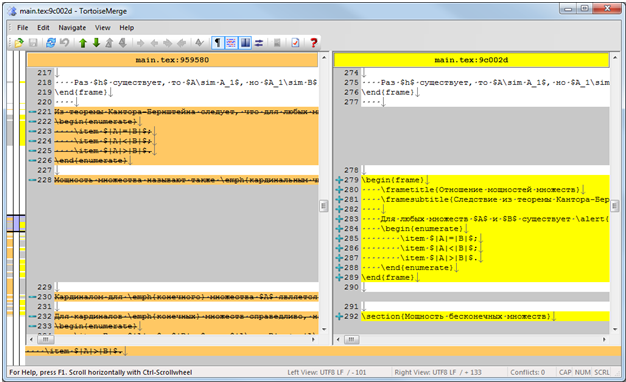
\includegraphics[width=0.8\textwidth]{pict/git}
    \end{center}
\end{frame}


\begin{frame}
\frametitle{Инструменты}
Издательские системы \LaTeX\ (компилятор, утилиты).
\begin{itemize}
    \item Windows
    \begin{itemize}
        \item MiK\TeX.
        \item \TeX\ Live.
    \end{itemize}
    \item Linux
    \begin{itemize}
        \item \TeX\ Live.
    \end{itemize}
    \item Mac
    \begin{itemize}
        \item Mac\TeX.
    \end{itemize}
\end{itemize}
Удобные редакторы исходных текстов: 
\begin{itemize}
    \item IDE Eclipse с плагином \TeX lipse.
    \item Редактор Emacs.
\end{itemize}
\end{frame}


\begin{frame}[fragile]
\frametitle{Класс}

\begin{center}
\verb"\documentclass[<настройки>]{<класс>}"
\end{center}

То, как будет \alert{оформлен} документ определяется его \alert{классом}. Существует множество классов, позволяющие создавать:
\begin{itemize}
    \item Статьи и сборники.
    \item Диссертации.
    \item Книги.
    \item Резюме.
    \item Презентации.
    \item Документы, следующие стандартам\footnote{Дипломы в соответствии с ЕСКД, заявления, стандартные формы}.
    \item и т.д.
\end{itemize}
\end{frame}


\begin{frame}[fragile]
\frametitle{Пакет}

\begin{center}
\verb"\usepackage[<настройки>]{<пакет>}"
\end{center}

Дополнительные \alert{возможности}\footnote{В виде дополнительных конструкций} поставляются в \alert{пакетах}. Существует множество пакетов, позволяющие:
\begin{itemize}
    \item Поддерживать различные кодировки исходного текста.
    \item Вставлять гиперссылки.
    \item Описывать таблицы, вставлять изображения, улучшать формулы.
    \item Писать стихи, пьесы, музыку и песни.
    \item Описывать электронные схемы.
    \item Описывать алгоритмы в псевдокоде.
    \item и т.д.
\end{itemize}
\end{frame}

Поиск пакетов с классами можно произвести на одном из архивов CTAN:


\subsection{CTAN}


\begin{frame}
\frametitle{CTAN}
\begin{definition}
    \alert{CTAN} (Comprehensive \TeX\ Archive Network) --- всеобъемлющая сеть архивов \TeX. Содержит архив классов, пакетов\footnote{Естественно, классы и пакеты хорошо документироаны в формате \TeX}, прикладных программ\footnote{Например, MiK\TeX\ может устанавливать необходимые для компиляции классы и пакеты из CTAN <<на лету>>}.
\end{definition}

Главный сайт \url{http://www.ctan.org/}\\
Огромное количество зеркал по всему миру.\\
Редиректор: \url{http://mirror.ctan.org/}.
\end{frame}

После установки можно найти классы и документацию на них в каталогах на собственном компьютере (показать). Так как \TeX --- это основной инструмент \TeX нического писателя, то вся документация представлена именно в формате \TeX.


\subsection{Компиляция}


Удельный вес информации об отображении в исходном тексте ничтожен --- он насыщен содержанием.


\begin{frame}[fragile]
\frametitle{Компиляция}
Исходный текст \LaTeX размещается в одном или нескольких файлах с расширением *.tex. Чтобы получить красиво \alert{оформленный} документ\footnote{Например, файл <<main.article.tex>> статьи этой презентации} требуется скомпилировать главный файл\footnote{Порядок вызова может быть и другим, например, если требуется построение библиографии программой bibtex}:

\begin{verbatim}
latex main.article.tex
latex main.article.tex
\end{verbatim}
Вы получите *.\alert{dvi} (\alert{d}e\alert{v}ice \alert{i}ndependent) файл документа.

Чтобы получить PDF версию используйте pdflatex:
\begin{verbatim}
pdflatex main.article.tex
pdflatex main.article.tex
\end{verbatim}
\end{frame}


Запуск происходит дважды, потому, что при первом запуске еще не сформирован *.aux файл с данными ссылок. Запуск может выглядеть и по-другому, например, если требуется построение библиографии программой bibtex.

\begin{frame}[fragile]
\frametitle{Компиляция}
\framesubtitle{Служебные файлы}
\begin{itemize}
    \item *.aux --- информация для перекрестного цитирования
    \item *.toc --- оглавление (\verb"\tableofcontents")
    \item *.lof --- список рисунков (\verb"\listoffigures")
    \item *.lot --- список таблиц (\verb"\listoftables")
    \item *.log --- лог
    \item \ldots
\end{itemize}
\end{frame}


\section{Синтаксис}


\subsection{Структура документа и секционирование}

\begin{frame}[fragile,allowframebreaks]
\frametitle{Структура исходного текста \LaTeX}
\begin{verbatim}
\documentclass{article} %указываем класс

%подключаем необходимые пакеты
\usepackage[utf8]{inputenc} %кодировка текста
\usepackage[russian]{babel} %поддержка русского языка
\usepackage{indentfirst} %у русских принято делать 
                         %отступ у первого абзаца

%глобальная настройка командами
\title{Структура \LaTeX\ документа} %название
\author{М.~М.~Шихов} %автор
\date{\today} %дата создания документа

\begin{document} %начало тела документа
    \maketitle %титульный лист
    \begin{abstract}Текст  аннотации.\end{abstract}
    \tableofcontents %оглавление,содержание
    \section{Заглавие первой секции}
    Текст первой секции, абзац первый.

    Текст первой секции, абзац второй.
    \subsection{Заглавие первой подсекции}
    Текст первой подсекции.
\end{document} %конец документа
\end{verbatim}
\end{frame}


\begin{frame}[fragile,allowframebreaks]
\frametitle{Команды, декларации, процедуры}
\begin{itemize}
\item \verb"{<body>}" --- область видимости.
\item \verb"\command[<settings>]{<arguments>}" --- команда.
    \begin{columns}
        \column{.48\textwidth}
            \begin{block}{Содержание}
                \verb"\emph{Логическое} ударение."\\
                \verb"Замечание\footnote{Примечание}"
            \end{block}
        
        \column{.48\textwidth}
            \begin{block}{Форма}
                \emph{Логическое} ударение.
                Замечание\footnote{Примечание}
            \end{block}
    \end{columns}

\item \verb"{\declaration[<settings>]}" --- декларация.
    \begin{columns}
        \column{.48\textwidth}
            \begin{block}{Содержание}
                \verb"{\em Логическое} ударение."\\
                \verb"{\bf Жирный} текст"
            \end{block}
        
        \column{.48\textwidth}
            \begin{block}{Форма}
                {\em Логическое} ударение.
                {\bf Жирный} текст
            \end{block}
    \end{columns}
    
\item \verb"\begin{command}[<settings>]<body>\end{command}" --- процедура.
    \begin{columns}
        \column{.48\textwidth}
            \begin{block}{Содержание}
                \begin{verbatim}
\begin{enumerate}                
    \item Раз элемент 
    \item Два элемент 
\end{enumerate}                
                \end{verbatim}
            \end{block}
        
        \column{.48\textwidth}
            \begin{block}{Форма}
                \begin{enumerate}                
                    \item Раз элемент 
                    \item Два элемент 
                \end{enumerate}                
            \end{block}
    \end{columns}

\end{itemize}
\begin{verbatim}
\end{verbatim}
\end{frame}


\begin{frame}[fragile,allowframebreaks]
    \frametitle{Собственные команды}

    \newcommand{\MyBinaryAdditionTask}[3]{
      Ссмложить целые числа A={#1} и B={#2} в \emph{двоичной} 
      системе счисления, в {#3}, в 8 разрядной сетке, 
      где 7-й разряд является знаковым.
    }
    
Например, перед телом документа объявим собственную команду:
\begin{semiverbatim}  
\\newcommand\{\alert{\\MyBinaryAdditionTask}\}[\alert{3}]\{
  С\alert{см}ложить целые числа A=\{\alert{\#1}\} и B=\{\alert{\#2}\} в \\emph\{двоичной\} 
  системе счисления, в \{\alert{\#3}\}, в 8 разрядной сетке, где 7-й 
  разряд является знаковым.
\}  
\end{semiverbatim}    

И используем много раз в тексте\footnote{Опечатку <<Ссмложить>> нужно исправить в \alert{одном} месте}:
\begin{semiverbatim}  
\\begin\{enumerate\}
    \\item \\MyBinaryAdditionTask\{10\}\{20\}\{ОК\}
    \\item \\MyBinaryAdditionTask\{20\}\{30\}\{ДК\}
    \\item \\MyBinaryAdditionTask\{30\}\{40\}\{ПК\}
    \\item \ldots
\\end\{enumerate\}
\end{semiverbatim}    

Получив следующий результат:
\begin{enumerate}
    \item \MyBinaryAdditionTask{10}{20}{ОК}
    \item \MyBinaryAdditionTask{20}{30}{ДК}
    \item \MyBinaryAdditionTask{30}{40}{ПК}
    \item \ldots
\end{enumerate}

\end{frame}


\begin{frame}[fragile]
\frametitle{Включения файлов}
Иногда бывает удобно разбить исходный текст на несколько частей, например по \alert{главам}, или выделить \alert{общие части} двух печатных документов. Это можно сделать с помощью команды
\begin{verbatim}
\input{<относительный путь к файлу>}
%расширение *.tex в имени файла указывать не надо
\end{verbatim}
Например, главный файл презентации main.beamer.tex так включает общую часть main.tex:
\begin{verbatim}
\documentclass[ignorenonframetext,red,utf8]{beamer}
\input{main}
\end{verbatim}
\end{frame}


\begin{frame}[fragile]
\frametitle{Секционирование}
%\verbatiminput{mathml/discriminant.xml}
\begin{verbatim}
\part        [<toc>]{<head>}
\chapter     [<toc>]{<head>}
\section     [<toc>]{<head>}
\subsection  [<toc>]{<head>}
\paragraph   [<toc>]{<head>}
\subparagraph[<toc>]{<head>}
\end{verbatim}
Текст \alert{toc} заносится в оглавление и колонтитулы, а \alert{head} в заголовок.
\end{frame}


\subsection{Формулы}

Рассказать о MathML, как об аналоге \LaTeX формул.
\begin{frame}[fragile]
\frametitle{Дискриминант: $x = \frac{-b \pm \sqrt{b^2 - 4ac}}{2a}$}
\framesubtitle{MathML}
%\verbatiminput{mathml/discriminant.xml}
\begin{verbatim}
<math xmlns="http://www.w3.org/1998/Math/MathML">
  <mrow><mi>x</mi><mo>=</mo>
    <mfrac><mrow> 
      <mrow><mo>-</mo><mi>b</mi></mrow>
      <mo>&#xB1;<!--PLUS-MINUS SIGN--></mo>
      <msqrt><mrow>
        <msup><mi>b</mi><mn>2</mn></msup><mo>-</mo>
        <mrow><mn>4</mn><mi>a</mi><mi>c</mi></mrow>
      </mrow></msqrt>
    </mrow><mrow><mn>2</mn><mi>a</mi></mrow>
  </mfrac></mrow>
</math>
\end{verbatim}
\end{frame}


\begin{frame}[fragile]
\frametitle{Дискриминант: $x = \frac{-b \pm \sqrt{b^2 - 4ac}}{2a}$}
\framesubtitle{\LaTeX}
\begin{verbatim}
x = \frac{-b \pm \sqrt{b^2 - 4ac}}{2a}
\end{verbatim}
\end{frame}


\begin{frame}[fragile]
\frametitle{Примеры формул \LaTeX}
\begin{itemize}
    
\item Операции $\sum,\prod,\bigcap,\int,\ldots$ (\verb"\sum,\prod,\bigcap,\int,"\ldots)
    \begin{columns}
        \column{.48\textwidth}
            \begin{block}{Содержание}
\begin{verbatim}
S=\sum_{i=1}^{N}a_0\cdot b^i
\end{verbatim}
            \end{block}
        
        \column{.48\textwidth}
            \begin{block}{Форма}
\[
S=\sum_{i=1}^{N}a_0\cdot b^i
\]
            \end{block}
    \end{columns}

\item Скобки и стрелки $\lfloor, \lceil, \{, \to,\ldots$ (\verb"\lfloor,\lceil,\{,\to"\ldots)
    \begin{columns}
        \column{.48\textwidth}
            \begin{block}{Содержание}
\begin{verbatim}
\delta=\langle 
    s_1\to \omega_1,\ldots,
    s_N\to \omega_N
\rangle
\end{verbatim}
            \end{block}
        
        \column{.48\textwidth}
            \begin{block}{Форма}
\[\delta=\langle 
    s_1\to \omega_1,\ldots,
    s_N\to \omega_N
\rangle\]
            \end{block}
    \end{columns}

\end{itemize}
\end{frame}


\begin{frame}[fragile]
\frametitle{Примеры формул \LaTeX}
\begin{itemize}
    
\item Дроби $\frac{\partial f}{\partial x}$ (\verb"\frac{\partial f}{\partial x}")
    \begin{columns}
        \column{.48\textwidth}
            \begin{block}{Содержание}
\begin{verbatim}
m=\frac{1}{
    1+\frac{1}{
        1+\frac{1}{n}
    }
}
\end{verbatim}
            \end{block}
        
        \column{.48\textwidth}
            \begin{block}{Форма}
\[
m=\frac{1}{1+\frac{1}{1+\frac{1}{n}}}
\]
            \end{block}
    \end{columns}

\item Отношения $\ne,\leq,\geq,\approx,\not\approx,\equiv,\not\equiv,\ldots$ 
(\verb"\ne,\leq,\geq,\approx,\not\approx,\equiv,\not\equiv,"\ldots)
    \begin{columns}
        \column{.48\textwidth}
            \begin{block}{Содержание}
\begin{verbatim}
x\approx\sqrt{y+\sqrt[3]{z+1}}
\end{verbatim}
            \end{block}
        
        \column{.48\textwidth}
            \begin{block}{Форма}
\[x\approx\sqrt{y+\sqrt[3]{z+1}}\]
            \end{block}
    \end{columns}

\end{itemize}
\end{frame}


\begin{frame}[fragile]
\frametitle{Примеры формул \LaTeX}
\begin{itemize}

\item Стрелки и пояснения $\vec{a}\xrightarrow{\lambda}\vec{b}$ (\verb"\vec{a}\xrightarrow{\lambda}\vec{b}")
    \begin{columns}
        \column{.48\textwidth}
            \begin{block}{Содержание}
\begin{verbatim}
p_0 =\underbrace{
    H(H(\cdots H(S)\cdots )) 
}_{N+1}
\end{verbatim}
            \end{block}
        
        \column{.48\textwidth}
            \begin{block}{Форма}
\[p_0 =\underbrace{
    H(H(\cdots H(S)\cdots )) 
}_{N+1}
\]
            \end{block}
    \end{columns}
    
\item Кириллица в текстовой моде (востребовано у экономистов)
    \begin{columns}
        \column{.48\textwidth}
            \begin{block}{Содержание}
\begin{verbatim}
S_\text{приб}=
S_\text{дох}-S_\text{расх}
\end{verbatim}
            \end{block}
        
        \column{.48\textwidth}
            \begin{block}{Форма}
\[S_\text{приб}=S_\text{дох}-S_\text{расх}\]
            \end{block}
    \end{columns}
   
\end{itemize}
\end{frame}


\begin{frame}[fragile]
\frametitle{Примеры формул \LaTeX}
\begin{itemize}

\item Матрицы
    \begin{columns}
        \column{.48\textwidth}
            \begin{block}{Содержание}
\begin{verbatim}
\left(\begin{array}{cc}
    a_{11} & a_{12}\\
    a_{21} & a_{22}\\
\end{array}\right)
\begin{pmatrix}
    x_1\\x_2
\end{pmatrix}=
\begin{pmatrix}
    b_1\\b_2
\end{pmatrix}
\end{verbatim}
            \end{block}
        
        \column{.48\textwidth}
            \begin{block}{Форма}
\[
\left(\begin{array}{cc}
a_{11} & a_{12}\\
a_{21} & a_{22}\\
\end{array}\right)
\begin{pmatrix}x_1\\x_2\end{pmatrix}=
\begin{pmatrix}b_1\\b_2\end{pmatrix}
\]
            \end{block}
    \end{columns}
    
\end{itemize}
\end{frame}



\begin{frame}[fragile]
\frametitle{Примеры формул \LaTeX}
\begin{itemize}

\item Логика $\forall,\exists,\lor,\land,\lnot,\ldots$ (\verb"\forall,\exists,\lor,\land,\lnot,"\ldots)
    \begin{columns}
        \column{.48\textwidth}
            \begin{block}{Содержание}
\begin{verbatim}
Q^l=\bigvee_{t=1}^{T}Q_t, 
Q_t=\tilde{q_t}\land q_t
\end{verbatim}
            \end{block}
        
        \column{.48\textwidth}
            \begin{block}{Форма}
            \[Q^l=\bigvee_{t=1}^{T}Q_t, Q_t=\tilde{q_t}\land q_t\]
            \end{block}
    \end{columns}
\end{itemize}
\end{frame}


\begin{frame}[fragile, allowframebreaks]
\frametitle{Варианты размещения формул в тексте}
\begin{example}[Содержание]
\begin{verbatim}
Можно разместить формулу в тексте $c=\sqrt{a^2+b^2}$. 
Можно сделать её выносной \[c=\sqrt{a^2+b^2}.\] 
Можно сделать её нумерованной и ссылаться на нее:
\begin{equation}
    \label{eq:pifagor}
    c=\sqrt{a^2+b^2}
\end{equation}
вот так: (\ref{eq:pifagor}) или \eqref{eq:pifagor}.
\end{verbatim}
\end{example}

\begin{example}[Форма]
Можно разместить формулу в тексте $c=\sqrt{a^2+b^2}$. 
Можно сделать её выносной \[c=\sqrt{a^2+b^2}.\] 
Можно сделать её нумерованной и ссылаться на нее:
\begin{equation}\label{eq:pifagor}
c=\sqrt{a^2+b^2}\end{equation}
вот так: (\ref{eq:pifagor}) или \eqref{eq:pifagor}.
\end{example}

\end{frame}


\subsection{Ссылки}


На все, что имеет номер, можно сослаться. Например, на элементы нумерованных списков, формулы, секции, рисунки, таблицы и т.д.

\begin{frame}[fragile,allowframebreaks]
\frametitle{Ссылки на пункты перечислений}
\begin{example}[Содержание]
\begin{verbatim}
\begin{enumerate}
    \item\label{enumer:haffSort} 
    События сортируются по убыванию вероятности.
    
    \item\label{enumer:haffGlue} 
    Два события с минимальными вероятностями объединяются в 
    одно составное событие c суммарной вероятностью исходных.
    
    \item Шаги \ref{enumer:haffSort} и \ref{enumer:haffGlue} 
    последовательно повторяются до тех пор, пока все события 
    не склеятся в единственное составное событие.
\end{enumerate}
\end{verbatim}
\end{example}

\begin{example}[Форма]
\begin{enumerate}
    \item\label{enumer:haffSort} 
    События сортируются по убыванию вероятности.
    
    \item\label{enumer:haffGlue} 
    Два события с минимальными вероятностями объединяются 
    в одно составное событие c суммарной вероятностью исходных.
    
    \item Шаги \ref{enumer:haffSort} и \ref{enumer:haffGlue} 
    последовательно повторяются до тех пор, пока все события 
    не склеятся в единственное составное событие.
\end{enumerate}
\end{example}
\end{frame}


\begin{frame}[fragile,allowframebreaks]
\frametitle{Ссылки на рисунки}
\begin{example}[Содержание]
\begin{verbatim}
\begin{figure}
    \begin{center}
        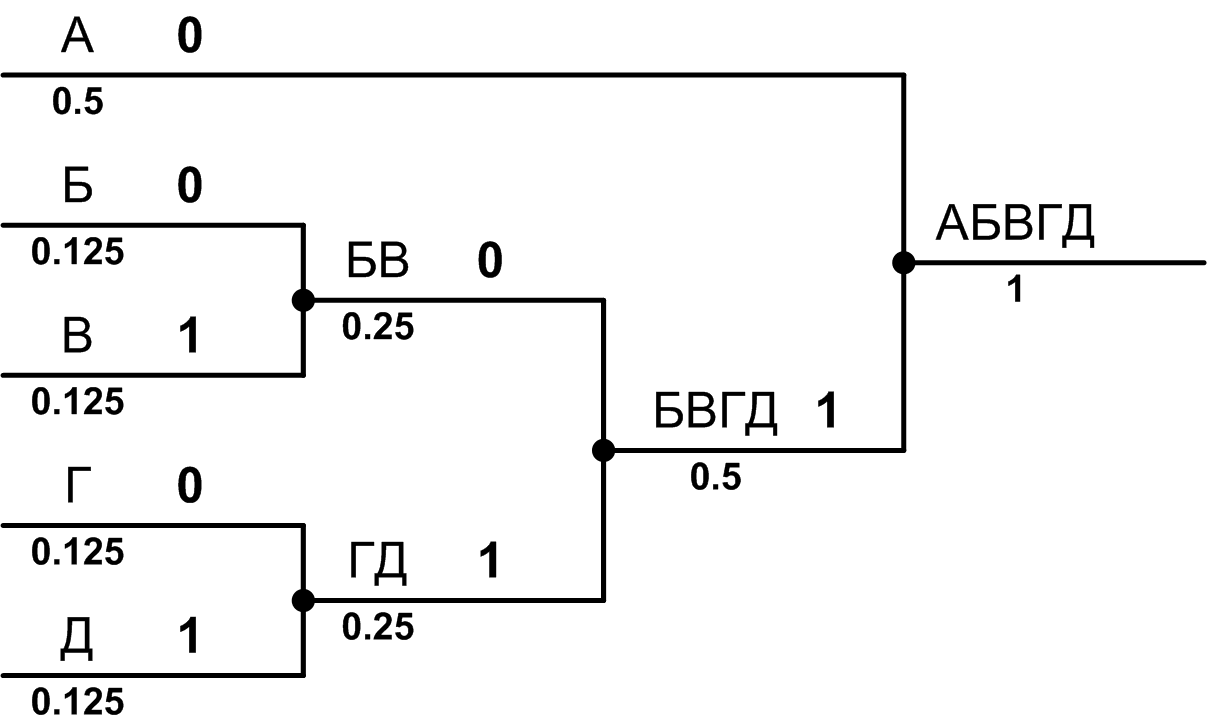
\includegraphics[height=0.2\textwidth]{pict/huffman}
        \caption{Алгоритм Хаффмана: кодирование}
        \label{pict:huffman}
    \end{center}
\end{figure} 
См. рисунок \ref{pict:huffman}
\end{verbatim}
\end{example}

\begin{example}[Форма]
\begin{figure}
    \begin{center}
        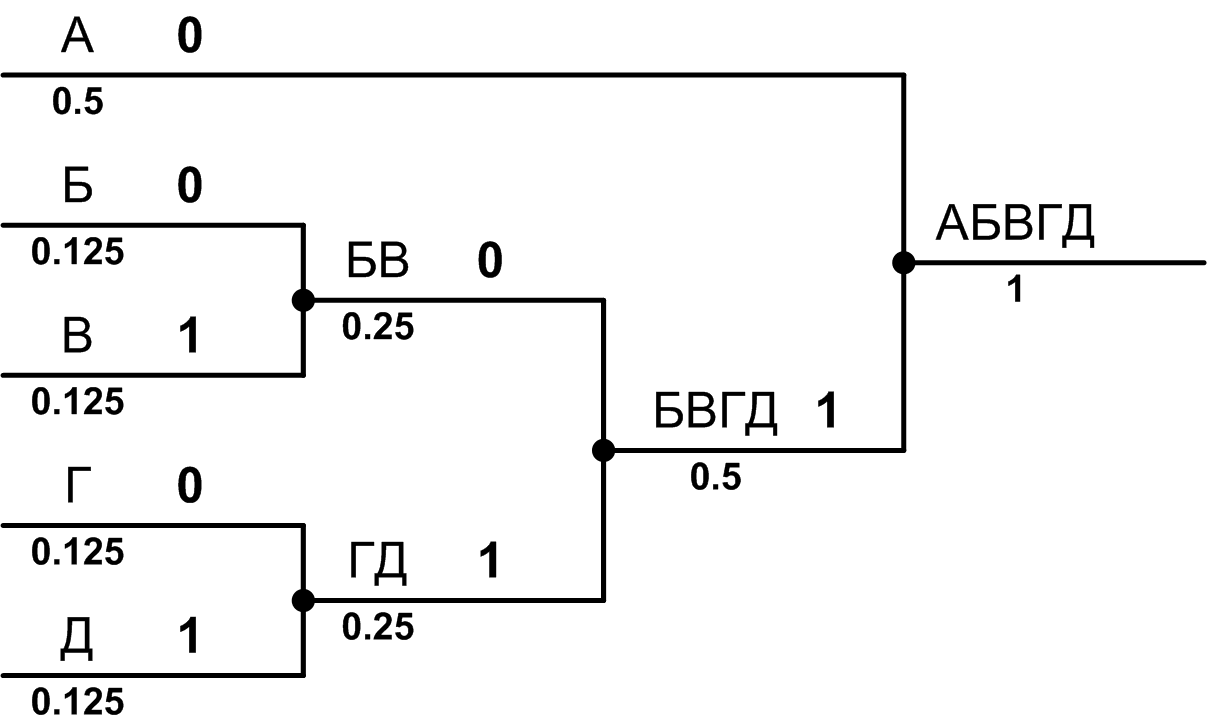
\includegraphics[height=0.2\textwidth]{pict/huffman}
        \caption{Алгоритм Хаффмана: кодирование}\label{pict:huffman}
    \end{center}
\end{figure} 
См. рисунок \ref{pict:huffman}
\end{example}
\end{frame}


\begin{frame}[fragile,allowframebreaks]
\frametitle{Ссылки на таблицы}
\begin{example}[Содержание]
\begin{verbatim}
\begin{table}[ht]   \caption{Пример таблицы}
                    \label{t:pifagor}
    \begin{tabular}[c]{|l|l|l|}
        \hline\hline
        $a$ & $b$ & \rotatebox{90}{$c=\sqrt{a^2+b^2}$}\\ 
        \hline\hline
        3   & 4   & 5          \\ \hline
        4   & 5   & $\sqrt{41}$\\ \hline
    \end{tabular}
\end{table}
См. таблицу \ref{t:pifagor}
\end{verbatim}
\end{example}

\begin{example}[Форма]
\begin{table}[ht]
\caption{Пример таблицы}\label{t:pifagor}
\centering
\begin{tabular}[c]{|l|l|l|}
\hline\hline
$a$ & $b$ & \rotatebox{90}{$c=\sqrt{a^2+b^2}$}\\ 
\hline\hline
3   & 4   & 5          \\ \hline
4   & 5   & $\sqrt{41}$\\ \hline
\end{tabular}
\end{table}
См. таблицу \ref{t:pifagor}
\end{example}
\end{frame}


\begin{frame}[fragile,allowframebreaks]
\frametitle{Ссылки}
\framesubtitle{Литература}
\begin{example}[Содержание]
\begin{verbatim}
Из книг по \LaTeXe\ можно рекомендовать 
\cite{bib:cotelnikov,bib:baldin}.
* * *
\begin{thebibliography}{99}
    \bibitem{bib:cotelnikov} Игорь Котельников,...
    \bibitem{bib:baldin} Балдин Е.М., Компьютерная,...
    * * *
\end{thebibliography}
\end{verbatim}
\end{example}

\begin{example}[Форма]
Из книг по \LaTeXe\ можно рекомендовать \cite{bib:cotelnikov,bib:baldin}.
\end{example}
\end{frame}

\begin{frame}[fragile,allowframebreaks]
    \frametitle{Ссылки на литературу правильно}
    \framesubtitle{bibtex}
    Заведём файл библиографии \verb"bibliobase.bib", содержащий записи о:
\begin{semiverbatim}  
%книгах:
@book\{bib:cotelnikov,
    author = \{И.Котельников and П.Чеботаев\},
    title = \{\{\\LaTeX\} по-русски\},
    publisher = \{Сибирский хронограф\},
    address = \{Новосибирск\},
    numpages = \{496\},
    language=\{russian\},
    year = \{2009\}
\}
\end{semiverbatim}  

\begin{semiverbatim}  
% статьях в журналах
@article\{kn:knuth:mf3,
    author = \{D. E. Knuth\},
    title = \{The New Versions of \{\\TeX\} and \{\\MF\}\},
    journal = \{TUGboat, the \{\\TeX\} User's Group Newsletter\},
    volume = 10,
    number = 3,
    pages = \{325--328\},
    month = \{nov\},
    year = 1989
\} 
\end{semiverbatim}  

\begin{semiverbatim}  
% интернет ссылках и прочем...
@misc\{bib:ctan,
    author = \{\},
    howpublished=\{\\url\{http://ctan.org/\}\},
    language=\{russian\},
    title = \{Comprehensive \{\\TeX\} Archive Network\}
\}
\end{semiverbatim}  

Теперь, чтобы возложить работу на плечи \verb"bibtex", следует вместо окружения \verb"thebibliography" использовать пару команд:
\begin{semiverbatim}  
\\bibliographystyle\{<имя стиля оформления библиографии>\}
\\bibliography\{<путь к файлу в формате bibtex>\}
\end{semiverbatim}  

\end{frame}


\appendix

\begin{frame}[allowframebreaks]{Библиография}
\begin{thebibliography}{99}
    \bibitem{bib:cotelnikov} Игорь Котельников, Платон Чеботаев, <<\LaTeX по-русски>>
    \bibitem{bib:baldin} Балдин Е.М., Компьютерная типография \LaTeX
    \bibitem{bib:knuthAllAbout} Дональд Э. Кнут, Все про \TeX
    \bibitem{bib:knuthTypograph} Дональд Э. Кнут, Компьютерная типография
\end{thebibliography}
\end{frame}


\end{document}

\end{verbatim}
\end{frame}


\begin{frame}[fragile]
\frametitle{Секционирование}
%\verbatiminput{mathml/discriminant.xml}
\begin{verbatim}
\part        [<toc>]{<head>}
\chapter     [<toc>]{<head>}
\section     [<toc>]{<head>}
\subsection  [<toc>]{<head>}
\paragraph   [<toc>]{<head>}
\subparagraph[<toc>]{<head>}
\end{verbatim}
Текст \alert{toc} заносится в оглавление и колонтитулы, а \alert{head} в заголовок.
\end{frame}


\subsection{Формулы}

Рассказать о MathML, как об аналоге \LaTeX формул.
\begin{frame}[fragile]
\frametitle{Дискриминант: $x = \frac{-b \pm \sqrt{b^2 - 4ac}}{2a}$}
\framesubtitle{MathML}
%\verbatiminput{mathml/discriminant.xml}
\begin{verbatim}
<math xmlns="http://www.w3.org/1998/Math/MathML">
  <mrow><mi>x</mi><mo>=</mo>
    <mfrac><mrow> 
      <mrow><mo>-</mo><mi>b</mi></mrow>
      <mo>&#xB1;<!--PLUS-MINUS SIGN--></mo>
      <msqrt><mrow>
        <msup><mi>b</mi><mn>2</mn></msup><mo>-</mo>
        <mrow><mn>4</mn><mi>a</mi><mi>c</mi></mrow>
      </mrow></msqrt>
    </mrow><mrow><mn>2</mn><mi>a</mi></mrow>
  </mfrac></mrow>
</math>
\end{verbatim}
\end{frame}


\begin{frame}[fragile]
\frametitle{Дискриминант: $x = \frac{-b \pm \sqrt{b^2 - 4ac}}{2a}$}
\framesubtitle{\LaTeX}
\begin{verbatim}
x = \frac{-b \pm \sqrt{b^2 - 4ac}}{2a}
\end{verbatim}
\end{frame}


\begin{frame}[fragile]
\frametitle{Примеры формул \LaTeX}
\begin{itemize}
    
\item Операции $\sum,\prod,\bigcap,\int,\ldots$ (\verb"\sum,\prod,\bigcap,\int,"\ldots)
    \begin{columns}
        \column{.48\textwidth}
            \begin{block}{Содержание}
\begin{verbatim}
S=\sum_{i=1}^{N}a_0\cdot b^i
\end{verbatim}
            \end{block}
        
        \column{.48\textwidth}
            \begin{block}{Форма}
\[
S=\sum_{i=1}^{N}a_0\cdot b^i
\]
            \end{block}
    \end{columns}

\item Скобки и стрелки $\lfloor, \lceil, \{, \to,\ldots$ (\verb"\lfloor,\lceil,\{,\to"\ldots)
    \begin{columns}
        \column{.48\textwidth}
            \begin{block}{Содержание}
\begin{verbatim}
\delta=\langle 
    s_1\to \omega_1,\ldots,
    s_N\to \omega_N
\rangle
\end{verbatim}
            \end{block}
        
        \column{.48\textwidth}
            \begin{block}{Форма}
\[\delta=\langle 
    s_1\to \omega_1,\ldots,
    s_N\to \omega_N
\rangle\]
            \end{block}
    \end{columns}

\end{itemize}
\end{frame}


\begin{frame}[fragile]
\frametitle{Примеры формул \LaTeX}
\begin{itemize}
    
\item Дроби $\frac{\partial f}{\partial x}$ (\verb"\frac{\partial f}{\partial x}")
    \begin{columns}
        \column{.48\textwidth}
            \begin{block}{Содержание}
\begin{verbatim}
m=\frac{1}{
    1+\frac{1}{
        1+\frac{1}{n}
    }
}
\end{verbatim}
            \end{block}
        
        \column{.48\textwidth}
            \begin{block}{Форма}
\[
m=\frac{1}{1+\frac{1}{1+\frac{1}{n}}}
\]
            \end{block}
    \end{columns}

\item Отношения $\ne,\leq,\geq,\approx,\not\approx,\equiv,\not\equiv,\ldots$ 
(\verb"\ne,\leq,\geq,\approx,\not\approx,\equiv,\not\equiv,"\ldots)
    \begin{columns}
        \column{.48\textwidth}
            \begin{block}{Содержание}
\begin{verbatim}
x\approx\sqrt{y+\sqrt[3]{z+1}}
\end{verbatim}
            \end{block}
        
        \column{.48\textwidth}
            \begin{block}{Форма}
\[x\approx\sqrt{y+\sqrt[3]{z+1}}\]
            \end{block}
    \end{columns}

\end{itemize}
\end{frame}


\begin{frame}[fragile]
\frametitle{Примеры формул \LaTeX}
\begin{itemize}

\item Стрелки и пояснения $\vec{a}\xrightarrow{\lambda}\vec{b}$ (\verb"\vec{a}\xrightarrow{\lambda}\vec{b}")
    \begin{columns}
        \column{.48\textwidth}
            \begin{block}{Содержание}
\begin{verbatim}
p_0 =\underbrace{
    H(H(\cdots H(S)\cdots )) 
}_{N+1}
\end{verbatim}
            \end{block}
        
        \column{.48\textwidth}
            \begin{block}{Форма}
\[p_0 =\underbrace{
    H(H(\cdots H(S)\cdots )) 
}_{N+1}
\]
            \end{block}
    \end{columns}
    
\item Кириллица в текстовой моде (востребовано у экономистов)
    \begin{columns}
        \column{.48\textwidth}
            \begin{block}{Содержание}
\begin{verbatim}
S_\text{приб}=
S_\text{дох}-S_\text{расх}
\end{verbatim}
            \end{block}
        
        \column{.48\textwidth}
            \begin{block}{Форма}
\[S_\text{приб}=S_\text{дох}-S_\text{расх}\]
            \end{block}
    \end{columns}
   
\end{itemize}
\end{frame}


\begin{frame}[fragile]
\frametitle{Примеры формул \LaTeX}
\begin{itemize}

\item Матрицы
    \begin{columns}
        \column{.48\textwidth}
            \begin{block}{Содержание}
\begin{verbatim}
\left(\begin{array}{cc}
    a_{11} & a_{12}\\
    a_{21} & a_{22}\\
\end{array}\right)
\begin{pmatrix}
    x_1\\x_2
\end{pmatrix}=
\begin{pmatrix}
    b_1\\b_2
\end{pmatrix}
\end{verbatim}
            \end{block}
        
        \column{.48\textwidth}
            \begin{block}{Форма}
\[
\left(\begin{array}{cc}
a_{11} & a_{12}\\
a_{21} & a_{22}\\
\end{array}\right)
\begin{pmatrix}x_1\\x_2\end{pmatrix}=
\begin{pmatrix}b_1\\b_2\end{pmatrix}
\]
            \end{block}
    \end{columns}
    
\end{itemize}
\end{frame}



\begin{frame}[fragile]
\frametitle{Примеры формул \LaTeX}
\begin{itemize}

\item Логика $\forall,\exists,\lor,\land,\lnot,\ldots$ (\verb"\forall,\exists,\lor,\land,\lnot,"\ldots)
    \begin{columns}
        \column{.48\textwidth}
            \begin{block}{Содержание}
\begin{verbatim}
Q^l=\bigvee_{t=1}^{T}Q_t, 
Q_t=\tilde{q_t}\land q_t
\end{verbatim}
            \end{block}
        
        \column{.48\textwidth}
            \begin{block}{Форма}
            \[Q^l=\bigvee_{t=1}^{T}Q_t, Q_t=\tilde{q_t}\land q_t\]
            \end{block}
    \end{columns}
\end{itemize}
\end{frame}


\begin{frame}[fragile, allowframebreaks]
\frametitle{Варианты размещения формул в тексте}
\begin{example}[Содержание]
\begin{verbatim}
Можно разместить формулу в тексте $c=\sqrt{a^2+b^2}$. 
Можно сделать её выносной \[c=\sqrt{a^2+b^2}.\] 
Можно сделать её нумерованной и ссылаться на нее:
\begin{equation}
    \label{eq:pifagor}
    c=\sqrt{a^2+b^2}
\end{equation}
вот так: (\ref{eq:pifagor}) или \eqref{eq:pifagor}.
\end{verbatim}
\end{example}

\begin{example}[Форма]
Можно разместить формулу в тексте $c=\sqrt{a^2+b^2}$. 
Можно сделать её выносной \[c=\sqrt{a^2+b^2}.\] 
Можно сделать её нумерованной и ссылаться на нее:
\begin{equation}\label{eq:pifagor}
c=\sqrt{a^2+b^2}\end{equation}
вот так: (\ref{eq:pifagor}) или \eqref{eq:pifagor}.
\end{example}

\end{frame}


\subsection{Ссылки}


На все, что имеет номер, можно сослаться. Например, на элементы нумерованных списков, формулы, секции, рисунки, таблицы и т.д.

\begin{frame}[fragile,allowframebreaks]
\frametitle{Ссылки на пункты перечислений}
\begin{example}[Содержание]
\begin{verbatim}
\begin{enumerate}
    \item\label{enumer:haffSort} 
    События сортируются по убыванию вероятности.
    
    \item\label{enumer:haffGlue} 
    Два события с минимальными вероятностями объединяются в 
    одно составное событие c суммарной вероятностью исходных.
    
    \item Шаги \ref{enumer:haffSort} и \ref{enumer:haffGlue} 
    последовательно повторяются до тех пор, пока все события 
    не склеятся в единственное составное событие.
\end{enumerate}
\end{verbatim}
\end{example}

\begin{example}[Форма]
\begin{enumerate}
    \item\label{enumer:haffSort} 
    События сортируются по убыванию вероятности.
    
    \item\label{enumer:haffGlue} 
    Два события с минимальными вероятностями объединяются 
    в одно составное событие c суммарной вероятностью исходных.
    
    \item Шаги \ref{enumer:haffSort} и \ref{enumer:haffGlue} 
    последовательно повторяются до тех пор, пока все события 
    не склеятся в единственное составное событие.
\end{enumerate}
\end{example}
\end{frame}


\begin{frame}[fragile,allowframebreaks]
\frametitle{Ссылки на рисунки}
\begin{example}[Содержание]
\begin{verbatim}
\begin{figure}
    \begin{center}
        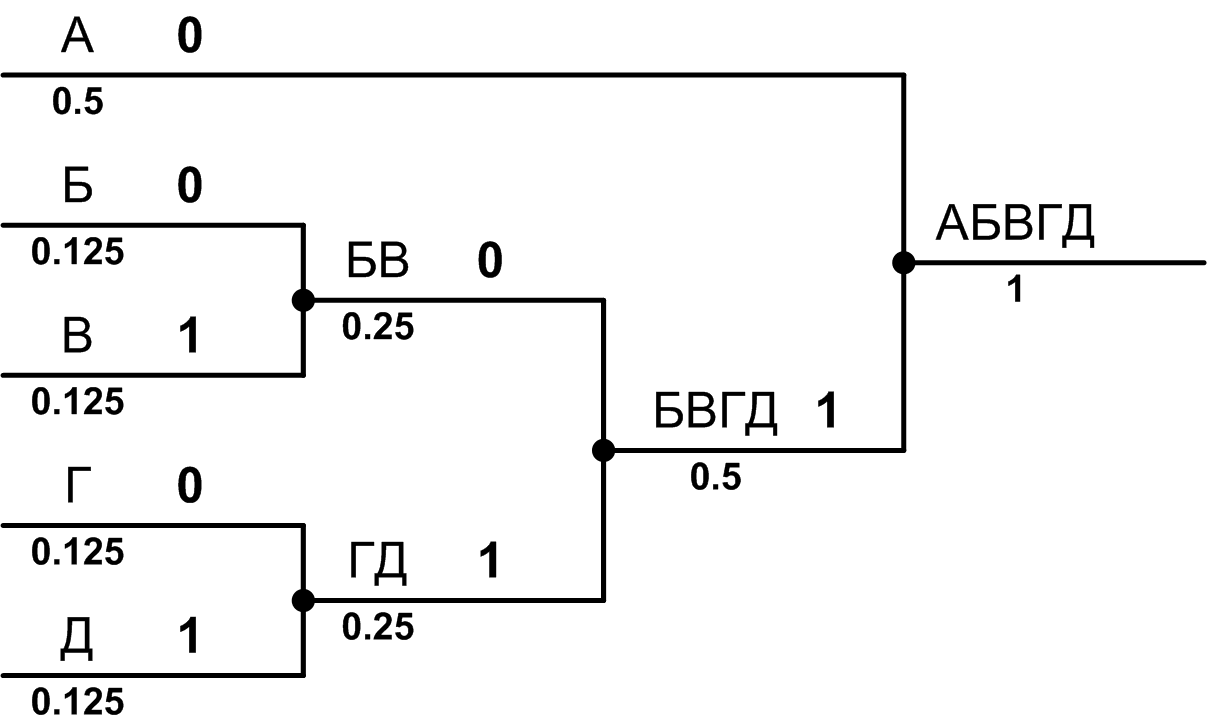
\includegraphics[height=0.2\textwidth]{pict/huffman}
        \caption{Алгоритм Хаффмана: кодирование}
        \label{pict:huffman}
    \end{center}
\end{figure} 
См. рисунок \ref{pict:huffman}
\end{verbatim}
\end{example}

\begin{example}[Форма]
\begin{figure}
    \begin{center}
        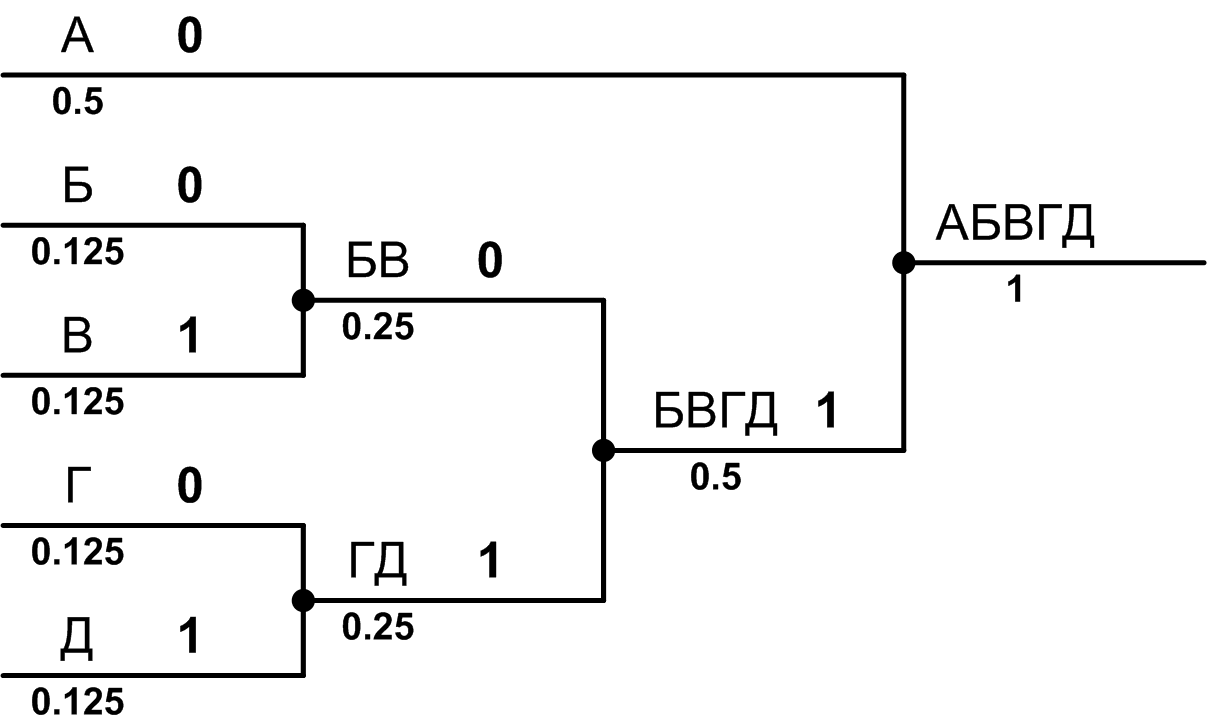
\includegraphics[height=0.2\textwidth]{pict/huffman}
        \caption{Алгоритм Хаффмана: кодирование}\label{pict:huffman}
    \end{center}
\end{figure} 
См. рисунок \ref{pict:huffman}
\end{example}
\end{frame}


\begin{frame}[fragile,allowframebreaks]
\frametitle{Ссылки на таблицы}
\begin{example}[Содержание]
\begin{verbatim}
\begin{table}[ht]   \caption{Пример таблицы}
                    \label{t:pifagor}
    \begin{tabular}[c]{|l|l|l|}
        \hline\hline
        $a$ & $b$ & \rotatebox{90}{$c=\sqrt{a^2+b^2}$}\\ 
        \hline\hline
        3   & 4   & 5          \\ \hline
        4   & 5   & $\sqrt{41}$\\ \hline
    \end{tabular}
\end{table}
См. таблицу \ref{t:pifagor}
\end{verbatim}
\end{example}

\begin{example}[Форма]
\begin{table}[ht]
\caption{Пример таблицы}\label{t:pifagor}
\centering
\begin{tabular}[c]{|l|l|l|}
\hline\hline
$a$ & $b$ & \rotatebox{90}{$c=\sqrt{a^2+b^2}$}\\ 
\hline\hline
3   & 4   & 5          \\ \hline
4   & 5   & $\sqrt{41}$\\ \hline
\end{tabular}
\end{table}
См. таблицу \ref{t:pifagor}
\end{example}
\end{frame}


\begin{frame}[fragile,allowframebreaks]
\frametitle{Ссылки}
\framesubtitle{Литература}
\begin{example}[Содержание]
\begin{verbatim}
Из книг по \LaTeXe\ можно рекомендовать 
\cite{bib:cotelnikov,bib:baldin}.
* * *
\begin{thebibliography}{99}
    \bibitem{bib:cotelnikov} Игорь Котельников,...
    \bibitem{bib:baldin} Балдин Е.М., Компьютерная,...
    * * *
\end{thebibliography}
\end{verbatim}
\end{example}

\begin{example}[Форма]
Из книг по \LaTeXe\ можно рекомендовать \cite{bib:cotelnikov,bib:baldin}.
\end{example}
\end{frame}

\begin{frame}[fragile,allowframebreaks]
    \frametitle{Ссылки на литературу правильно}
    \framesubtitle{bibtex}
    Заведём файл библиографии \verb"bibliobase.bib", содержащий записи о:
\begin{semiverbatim}  
%книгах:
@book\{bib:cotelnikov,
    author = \{И.Котельников and П.Чеботаев\},
    title = \{\{\\LaTeX\} по-русски\},
    publisher = \{Сибирский хронограф\},
    address = \{Новосибирск\},
    numpages = \{496\},
    language=\{russian\},
    year = \{2009\}
\}
\end{semiverbatim}  

\begin{semiverbatim}  
% статьях в журналах
@article\{kn:knuth:mf3,
    author = \{D. E. Knuth\},
    title = \{The New Versions of \{\\TeX\} and \{\\MF\}\},
    journal = \{TUGboat, the \{\\TeX\} User's Group Newsletter\},
    volume = 10,
    number = 3,
    pages = \{325--328\},
    month = \{nov\},
    year = 1989
\} 
\end{semiverbatim}  

\begin{semiverbatim}  
% интернет ссылках и прочем...
@misc\{bib:ctan,
    author = \{\},
    howpublished=\{\\url\{http://ctan.org/\}\},
    language=\{russian\},
    title = \{Comprehensive \{\\TeX\} Archive Network\}
\}
\end{semiverbatim}  

Теперь, чтобы возложить работу на плечи \verb"bibtex", следует вместо окружения \verb"thebibliography" использовать пару команд:
\begin{semiverbatim}  
\\bibliographystyle\{<имя стиля оформления библиографии>\}
\\bibliography\{<путь к файлу в формате bibtex>\}
\end{semiverbatim}  

\end{frame}


\appendix

\begin{frame}[allowframebreaks]{Библиография}
\begin{thebibliography}{99}
    \bibitem{bib:cotelnikov} Игорь Котельников, Платон Чеботаев, <<\LaTeX по-русски>>
    \bibitem{bib:baldin} Балдин Е.М., Компьютерная типография \LaTeX
    \bibitem{bib:knuthAllAbout} Дональд Э. Кнут, Все про \TeX
    \bibitem{bib:knuthTypograph} Дональд Э. Кнут, Компьютерная типография
\end{thebibliography}
\end{frame}


\end{document}

\end{verbatim}
\end{frame}


\begin{frame}[fragile]
\frametitle{Секционирование}
%\verbatiminput{mathml/discriminant.xml}
\begin{verbatim}
\part        [<toc>]{<head>}
\chapter     [<toc>]{<head>}
\section     [<toc>]{<head>}
\subsection  [<toc>]{<head>}
\paragraph   [<toc>]{<head>}
\subparagraph[<toc>]{<head>}
\end{verbatim}
Текст \alert{toc} заносится в оглавление и колонтитулы, а \alert{head} в заголовок.
\end{frame}


\subsection{Формулы}

Рассказать о MathML, как об аналоге \LaTeX формул.
\begin{frame}[fragile]
\frametitle{Дискриминант: $x = \frac{-b \pm \sqrt{b^2 - 4ac}}{2a}$}
\framesubtitle{MathML}
%\verbatiminput{mathml/discriminant.xml}
\begin{verbatim}
<math xmlns="http://www.w3.org/1998/Math/MathML">
  <mrow><mi>x</mi><mo>=</mo>
    <mfrac><mrow> 
      <mrow><mo>-</mo><mi>b</mi></mrow>
      <mo>&#xB1;<!--PLUS-MINUS SIGN--></mo>
      <msqrt><mrow>
        <msup><mi>b</mi><mn>2</mn></msup><mo>-</mo>
        <mrow><mn>4</mn><mi>a</mi><mi>c</mi></mrow>
      </mrow></msqrt>
    </mrow><mrow><mn>2</mn><mi>a</mi></mrow>
  </mfrac></mrow>
</math>
\end{verbatim}
\end{frame}


\begin{frame}[fragile]
\frametitle{Дискриминант: $x = \frac{-b \pm \sqrt{b^2 - 4ac}}{2a}$}
\framesubtitle{\LaTeX}
\begin{verbatim}
x = \frac{-b \pm \sqrt{b^2 - 4ac}}{2a}
\end{verbatim}
\end{frame}


\begin{frame}[fragile]
\frametitle{Примеры формул \LaTeX}
\begin{itemize}
    
\item Операции $\sum,\prod,\bigcap,\int,\ldots$ (\verb"\sum,\prod,\bigcap,\int,"\ldots)
    \begin{columns}
        \column{.48\textwidth}
            \begin{block}{Содержание}
\begin{verbatim}
S=\sum_{i=1}^{N}a_0\cdot b^i
\end{verbatim}
            \end{block}
        
        \column{.48\textwidth}
            \begin{block}{Форма}
\[
S=\sum_{i=1}^{N}a_0\cdot b^i
\]
            \end{block}
    \end{columns}

\item Скобки и стрелки $\lfloor, \lceil, \{, \to,\ldots$ (\verb"\lfloor,\lceil,\{,\to"\ldots)
    \begin{columns}
        \column{.48\textwidth}
            \begin{block}{Содержание}
\begin{verbatim}
\delta=\langle 
    s_1\to \omega_1,\ldots,
    s_N\to \omega_N
\rangle
\end{verbatim}
            \end{block}
        
        \column{.48\textwidth}
            \begin{block}{Форма}
\[\delta=\langle 
    s_1\to \omega_1,\ldots,
    s_N\to \omega_N
\rangle\]
            \end{block}
    \end{columns}

\end{itemize}
\end{frame}


\begin{frame}[fragile]
\frametitle{Примеры формул \LaTeX}
\begin{itemize}
    
\item Дроби $\frac{\partial f}{\partial x}$ (\verb"\frac{\partial f}{\partial x}")
    \begin{columns}
        \column{.48\textwidth}
            \begin{block}{Содержание}
\begin{verbatim}
m=\frac{1}{
    1+\frac{1}{
        1+\frac{1}{n}
    }
}
\end{verbatim}
            \end{block}
        
        \column{.48\textwidth}
            \begin{block}{Форма}
\[
m=\frac{1}{1+\frac{1}{1+\frac{1}{n}}}
\]
            \end{block}
    \end{columns}

\item Отношения $\ne,\leq,\geq,\approx,\not\approx,\equiv,\not\equiv,\ldots$ 
(\verb"\ne,\leq,\geq,\approx,\not\approx,\equiv,\not\equiv,"\ldots)
    \begin{columns}
        \column{.48\textwidth}
            \begin{block}{Содержание}
\begin{verbatim}
x\approx\sqrt{y+\sqrt[3]{z+1}}
\end{verbatim}
            \end{block}
        
        \column{.48\textwidth}
            \begin{block}{Форма}
\[x\approx\sqrt{y+\sqrt[3]{z+1}}\]
            \end{block}
    \end{columns}

\end{itemize}
\end{frame}


\begin{frame}[fragile]
\frametitle{Примеры формул \LaTeX}
\begin{itemize}

\item Стрелки и пояснения $\vec{a}\xrightarrow{\lambda}\vec{b}$ (\verb"\vec{a}\xrightarrow{\lambda}\vec{b}")
    \begin{columns}
        \column{.48\textwidth}
            \begin{block}{Содержание}
\begin{verbatim}
p_0 =\underbrace{
    H(H(\cdots H(S)\cdots )) 
}_{N+1}
\end{verbatim}
            \end{block}
        
        \column{.48\textwidth}
            \begin{block}{Форма}
\[p_0 =\underbrace{
    H(H(\cdots H(S)\cdots )) 
}_{N+1}
\]
            \end{block}
    \end{columns}
    
\item Кириллица в текстовой моде (востребовано у экономистов)
    \begin{columns}
        \column{.48\textwidth}
            \begin{block}{Содержание}
\begin{verbatim}
S_\text{приб}=
S_\text{дох}-S_\text{расх}
\end{verbatim}
            \end{block}
        
        \column{.48\textwidth}
            \begin{block}{Форма}
\[S_\text{приб}=S_\text{дох}-S_\text{расх}\]
            \end{block}
    \end{columns}
   
\end{itemize}
\end{frame}


\begin{frame}[fragile]
\frametitle{Примеры формул \LaTeX}
\begin{itemize}

\item Матрицы
    \begin{columns}
        \column{.48\textwidth}
            \begin{block}{Содержание}
\begin{verbatim}
\left(\begin{array}{cc}
    a_{11} & a_{12}\\
    a_{21} & a_{22}\\
\end{array}\right)
\begin{pmatrix}
    x_1\\x_2
\end{pmatrix}=
\begin{pmatrix}
    b_1\\b_2
\end{pmatrix}
\end{verbatim}
            \end{block}
        
        \column{.48\textwidth}
            \begin{block}{Форма}
\[
\left(\begin{array}{cc}
a_{11} & a_{12}\\
a_{21} & a_{22}\\
\end{array}\right)
\begin{pmatrix}x_1\\x_2\end{pmatrix}=
\begin{pmatrix}b_1\\b_2\end{pmatrix}
\]
            \end{block}
    \end{columns}
    
\end{itemize}
\end{frame}



\begin{frame}[fragile]
\frametitle{Примеры формул \LaTeX}
\begin{itemize}

\item Логика $\forall,\exists,\lor,\land,\lnot,\ldots$ (\verb"\forall,\exists,\lor,\land,\lnot,"\ldots)
    \begin{columns}
        \column{.48\textwidth}
            \begin{block}{Содержание}
\begin{verbatim}
Q^l=\bigvee_{t=1}^{T}Q_t, 
Q_t=\tilde{q_t}\land q_t
\end{verbatim}
            \end{block}
        
        \column{.48\textwidth}
            \begin{block}{Форма}
            \[Q^l=\bigvee_{t=1}^{T}Q_t, Q_t=\tilde{q_t}\land q_t\]
            \end{block}
    \end{columns}
\end{itemize}
\end{frame}


\begin{frame}[fragile, allowframebreaks]
\frametitle{Варианты размещения формул в тексте}
\begin{example}[Содержание]
\begin{verbatim}
Можно разместить формулу в тексте $c=\sqrt{a^2+b^2}$. 
Можно сделать её выносной \[c=\sqrt{a^2+b^2}.\] 
Можно сделать её нумерованной и ссылаться на нее:
\begin{equation}
    \label{eq:pifagor}
    c=\sqrt{a^2+b^2}
\end{equation}
вот так: (\ref{eq:pifagor}) или \eqref{eq:pifagor}.
\end{verbatim}
\end{example}

\begin{example}[Форма]
Можно разместить формулу в тексте $c=\sqrt{a^2+b^2}$. 
Можно сделать её выносной \[c=\sqrt{a^2+b^2}.\] 
Можно сделать её нумерованной и ссылаться на нее:
\begin{equation}\label{eq:pifagor}
c=\sqrt{a^2+b^2}\end{equation}
вот так: (\ref{eq:pifagor}) или \eqref{eq:pifagor}.
\end{example}

\end{frame}


\subsection{Ссылки}


На все, что имеет номер, можно сослаться. Например, на элементы нумерованных списков, формулы, секции, рисунки, таблицы и т.д.

\begin{frame}[fragile,allowframebreaks]
\frametitle{Ссылки на пункты перечислений}
\begin{example}[Содержание]
\begin{verbatim}
\begin{enumerate}
    \item\label{enumer:haffSort} 
    События сортируются по убыванию вероятности.
    
    \item\label{enumer:haffGlue} 
    Два события с минимальными вероятностями объединяются в 
    одно составное событие c суммарной вероятностью исходных.
    
    \item Шаги \ref{enumer:haffSort} и \ref{enumer:haffGlue} 
    последовательно повторяются до тех пор, пока все события 
    не склеятся в единственное составное событие.
\end{enumerate}
\end{verbatim}
\end{example}

\begin{example}[Форма]
\begin{enumerate}
    \item\label{enumer:haffSort} 
    События сортируются по убыванию вероятности.
    
    \item\label{enumer:haffGlue} 
    Два события с минимальными вероятностями объединяются 
    в одно составное событие c суммарной вероятностью исходных.
    
    \item Шаги \ref{enumer:haffSort} и \ref{enumer:haffGlue} 
    последовательно повторяются до тех пор, пока все события 
    не склеятся в единственное составное событие.
\end{enumerate}
\end{example}
\end{frame}


\begin{frame}[fragile,allowframebreaks]
\frametitle{Ссылки на рисунки}
\begin{example}[Содержание]
\begin{verbatim}
\begin{figure}
    \begin{center}
        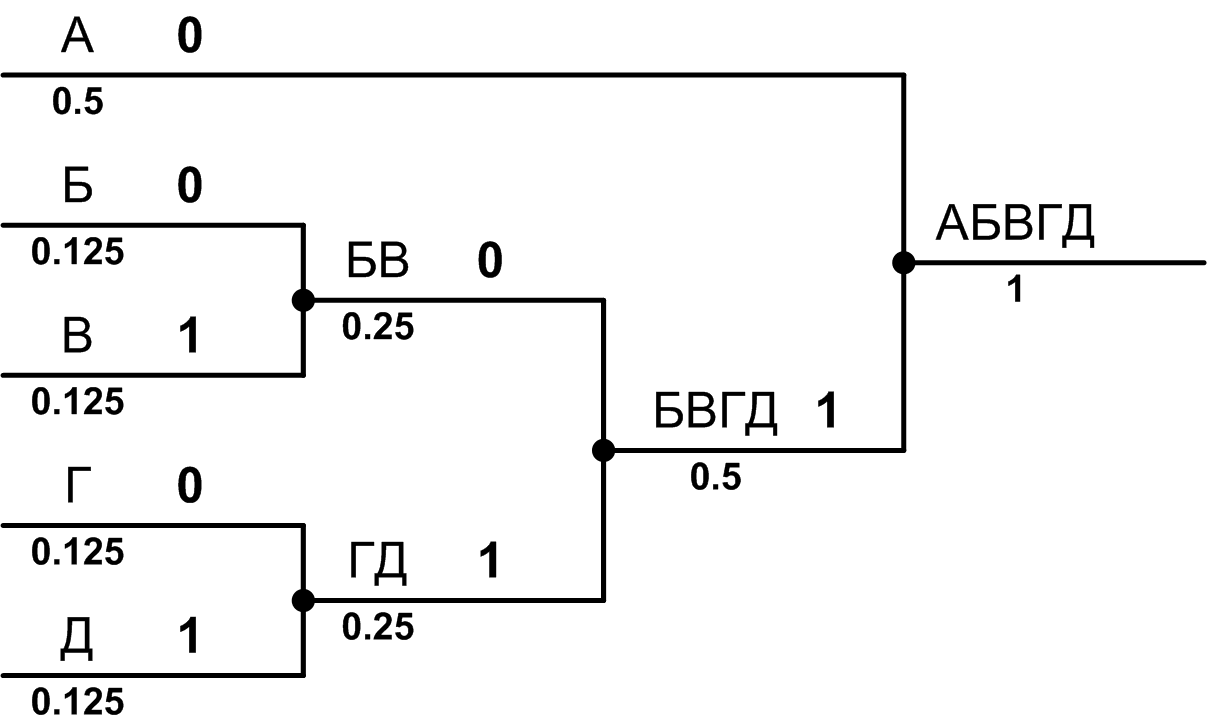
\includegraphics[height=0.2\textwidth]{pict/huffman}
        \caption{Алгоритм Хаффмана: кодирование}
        \label{pict:huffman}
    \end{center}
\end{figure} 
См. рисунок \ref{pict:huffman}
\end{verbatim}
\end{example}

\begin{example}[Форма]
\begin{figure}
    \begin{center}
        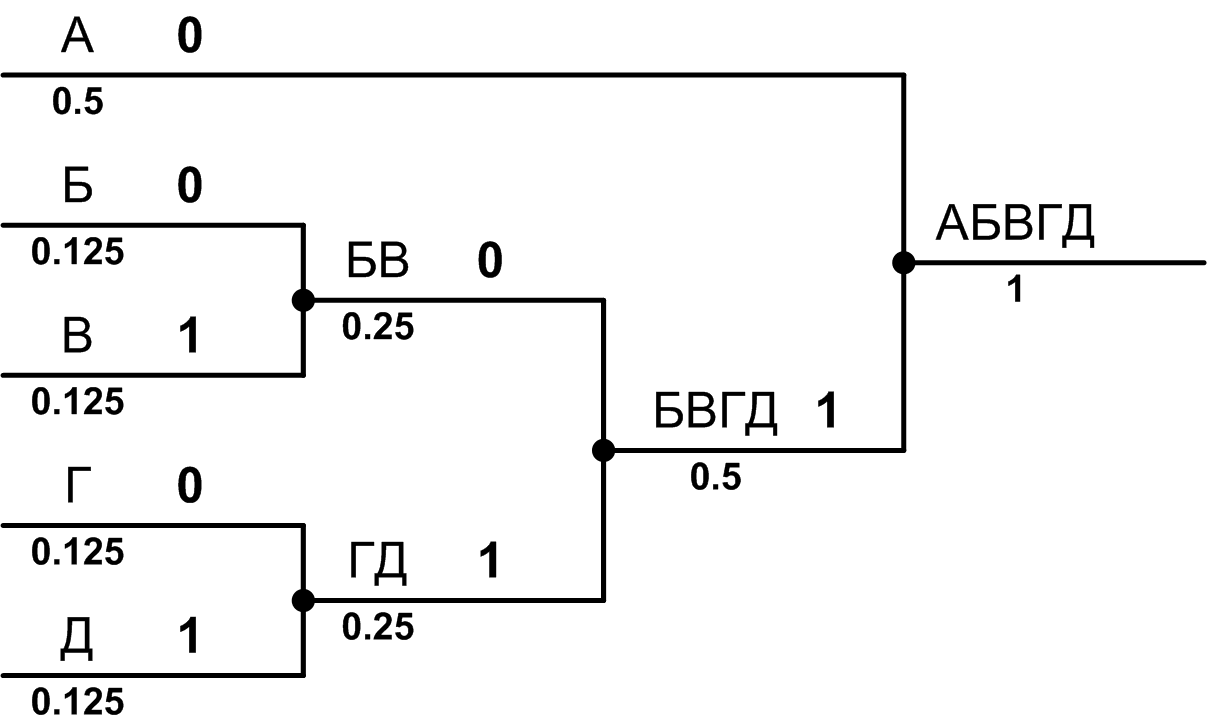
\includegraphics[height=0.2\textwidth]{pict/huffman}
        \caption{Алгоритм Хаффмана: кодирование}\label{pict:huffman}
    \end{center}
\end{figure} 
См. рисунок \ref{pict:huffman}
\end{example}
\end{frame}


\begin{frame}[fragile,allowframebreaks]
\frametitle{Ссылки на таблицы}
\begin{example}[Содержание]
\begin{verbatim}
\begin{table}[ht]   \caption{Пример таблицы}
                    \label{t:pifagor}
    \begin{tabular}[c]{|l|l|l|}
        \hline\hline
        $a$ & $b$ & \rotatebox{90}{$c=\sqrt{a^2+b^2}$}\\ 
        \hline\hline
        3   & 4   & 5          \\ \hline
        4   & 5   & $\sqrt{41}$\\ \hline
    \end{tabular}
\end{table}
См. таблицу \ref{t:pifagor}
\end{verbatim}
\end{example}

\begin{example}[Форма]
\begin{table}[ht]
\caption{Пример таблицы}\label{t:pifagor}
\centering
\begin{tabular}[c]{|l|l|l|}
\hline\hline
$a$ & $b$ & \rotatebox{90}{$c=\sqrt{a^2+b^2}$}\\ 
\hline\hline
3   & 4   & 5          \\ \hline
4   & 5   & $\sqrt{41}$\\ \hline
\end{tabular}
\end{table}
См. таблицу \ref{t:pifagor}
\end{example}
\end{frame}


\begin{frame}[fragile,allowframebreaks]
\frametitle{Ссылки}
\framesubtitle{Литература}
\begin{example}[Содержание]
\begin{verbatim}
Из книг по \LaTeXe\ можно рекомендовать 
\cite{bib:cotelnikov,bib:baldin}.
* * *
\begin{thebibliography}{99}
    \bibitem{bib:cotelnikov} Игорь Котельников,...
    \bibitem{bib:baldin} Балдин Е.М., Компьютерная,...
    * * *
\end{thebibliography}
\end{verbatim}
\end{example}

\begin{example}[Форма]
Из книг по \LaTeXe\ можно рекомендовать \cite{bib:cotelnikov,bib:baldin}.
\end{example}
\end{frame}

\begin{frame}[fragile,allowframebreaks]
    \frametitle{Ссылки на литературу правильно}
    \framesubtitle{bibtex}
    Заведём файл библиографии \verb"bibliobase.bib", содержащий записи о:
\begin{semiverbatim}  
%книгах:
@book\{bib:cotelnikov,
    author = \{И.Котельников and П.Чеботаев\},
    title = \{\{\\LaTeX\} по-русски\},
    publisher = \{Сибирский хронограф\},
    address = \{Новосибирск\},
    numpages = \{496\},
    language=\{russian\},
    year = \{2009\}
\}
\end{semiverbatim}  

\begin{semiverbatim}  
% статьях в журналах
@article\{kn:knuth:mf3,
    author = \{D. E. Knuth\},
    title = \{The New Versions of \{\\TeX\} and \{\\MF\}\},
    journal = \{TUGboat, the \{\\TeX\} User's Group Newsletter\},
    volume = 10,
    number = 3,
    pages = \{325--328\},
    month = \{nov\},
    year = 1989
\} 
\end{semiverbatim}  

\begin{semiverbatim}  
% интернет ссылках и прочем...
@misc\{bib:ctan,
    author = \{\},
    howpublished=\{\\url\{http://ctan.org/\}\},
    language=\{russian\},
    title = \{Comprehensive \{\\TeX\} Archive Network\}
\}
\end{semiverbatim}  

Теперь, чтобы возложить работу на плечи \verb"bibtex", следует вместо окружения \verb"thebibliography" использовать пару команд:
\begin{semiverbatim}  
\\bibliographystyle\{<имя стиля оформления библиографии>\}
\\bibliography\{<путь к файлу в формате bibtex>\}
\end{semiverbatim}  

\end{frame}


\appendix

\begin{frame}[allowframebreaks]{Библиография}
\begin{thebibliography}{99}
    \bibitem{bib:cotelnikov} Игорь Котельников, Платон Чеботаев, <<\LaTeX по-русски>>
    \bibitem{bib:baldin} Балдин Е.М., Компьютерная типография \LaTeX
    \bibitem{bib:knuthAllAbout} Дональд Э. Кнут, Все про \TeX
    \bibitem{bib:knuthTypograph} Дональд Э. Кнут, Компьютерная типография
\end{thebibliography}
\end{frame}


\end{document}

\end{verbatim}
\end{frame}


\begin{frame}[fragile]
\frametitle{Секционирование}
%\verbatiminput{mathml/discriminant.xml}
\begin{verbatim}
\part        [<toc>]{<head>}
\chapter     [<toc>]{<head>}
\section     [<toc>]{<head>}
\subsection  [<toc>]{<head>}
\paragraph   [<toc>]{<head>}
\subparagraph[<toc>]{<head>}
\end{verbatim}
Текст \alert{toc} заносится в оглавление и колонтитулы, а \alert{head} в заголовок.
\end{frame}


\subsection{Формулы}

Рассказать о MathML, как об аналоге \LaTeX формул.
\begin{frame}[fragile]
\frametitle{Дискриминант: $x = \frac{-b \pm \sqrt{b^2 - 4ac}}{2a}$}
\framesubtitle{MathML}
%\verbatiminput{mathml/discriminant.xml}
\begin{verbatim}
<math xmlns="http://www.w3.org/1998/Math/MathML">
  <mrow><mi>x</mi><mo>=</mo>
    <mfrac><mrow> 
      <mrow><mo>-</mo><mi>b</mi></mrow>
      <mo>&#xB1;<!--PLUS-MINUS SIGN--></mo>
      <msqrt><mrow>
        <msup><mi>b</mi><mn>2</mn></msup><mo>-</mo>
        <mrow><mn>4</mn><mi>a</mi><mi>c</mi></mrow>
      </mrow></msqrt>
    </mrow><mrow><mn>2</mn><mi>a</mi></mrow>
  </mfrac></mrow>
</math>
\end{verbatim}
\end{frame}


\begin{frame}[fragile]
\frametitle{Дискриминант: $x = \frac{-b \pm \sqrt{b^2 - 4ac}}{2a}$}
\framesubtitle{\LaTeX}
\begin{verbatim}
x = \frac{-b \pm \sqrt{b^2 - 4ac}}{2a}
\end{verbatim}
\end{frame}


\begin{frame}[fragile]
\frametitle{Примеры формул \LaTeX}
\begin{itemize}
    
\item Операции $\sum,\prod,\bigcap,\int,\ldots$ (\verb"\sum,\prod,\bigcap,\int,"\ldots)
    \begin{columns}
        \column{.48\textwidth}
            \begin{block}{Содержание}
\begin{verbatim}
S=\sum_{i=1}^{N}a_0\cdot b^i
\end{verbatim}
            \end{block}
        
        \column{.48\textwidth}
            \begin{block}{Форма}
\[
S=\sum_{i=1}^{N}a_0\cdot b^i
\]
            \end{block}
    \end{columns}

\item Скобки и стрелки $\lfloor, \lceil, \{, \to,\ldots$ (\verb"\lfloor,\lceil,\{,\to"\ldots)
    \begin{columns}
        \column{.48\textwidth}
            \begin{block}{Содержание}
\begin{verbatim}
\delta=\langle 
    s_1\to \omega_1,\ldots,
    s_N\to \omega_N
\rangle
\end{verbatim}
            \end{block}
        
        \column{.48\textwidth}
            \begin{block}{Форма}
\[\delta=\langle 
    s_1\to \omega_1,\ldots,
    s_N\to \omega_N
\rangle\]
            \end{block}
    \end{columns}

\end{itemize}
\end{frame}


\begin{frame}[fragile]
\frametitle{Примеры формул \LaTeX}
\begin{itemize}
    
\item Дроби $\frac{\partial f}{\partial x}$ (\verb"\frac{\partial f}{\partial x}")
    \begin{columns}
        \column{.48\textwidth}
            \begin{block}{Содержание}
\begin{verbatim}
m=\frac{1}{
    1+\frac{1}{
        1+\frac{1}{n}
    }
}
\end{verbatim}
            \end{block}
        
        \column{.48\textwidth}
            \begin{block}{Форма}
\[
m=\frac{1}{1+\frac{1}{1+\frac{1}{n}}}
\]
            \end{block}
    \end{columns}

\item Отношения $\ne,\leq,\geq,\approx,\not\approx,\equiv,\not\equiv,\ldots$ 
(\verb"\ne,\leq,\geq,\approx,\not\approx,\equiv,\not\equiv,"\ldots)
    \begin{columns}
        \column{.48\textwidth}
            \begin{block}{Содержание}
\begin{verbatim}
x\approx\sqrt{y+\sqrt[3]{z+1}}
\end{verbatim}
            \end{block}
        
        \column{.48\textwidth}
            \begin{block}{Форма}
\[x\approx\sqrt{y+\sqrt[3]{z+1}}\]
            \end{block}
    \end{columns}

\end{itemize}
\end{frame}


\begin{frame}[fragile]
\frametitle{Примеры формул \LaTeX}
\begin{itemize}

\item Стрелки и пояснения $\vec{a}\xrightarrow{\lambda}\vec{b}$ (\verb"\vec{a}\xrightarrow{\lambda}\vec{b}")
    \begin{columns}
        \column{.48\textwidth}
            \begin{block}{Содержание}
\begin{verbatim}
p_0 =\underbrace{
    H(H(\cdots H(S)\cdots )) 
}_{N+1}
\end{verbatim}
            \end{block}
        
        \column{.48\textwidth}
            \begin{block}{Форма}
\[p_0 =\underbrace{
    H(H(\cdots H(S)\cdots )) 
}_{N+1}
\]
            \end{block}
    \end{columns}
    
\item Кириллица в текстовой моде (востребовано у экономистов)
    \begin{columns}
        \column{.48\textwidth}
            \begin{block}{Содержание}
\begin{verbatim}
S_\text{приб}=
S_\text{дох}-S_\text{расх}
\end{verbatim}
            \end{block}
        
        \column{.48\textwidth}
            \begin{block}{Форма}
\[S_\text{приб}=S_\text{дох}-S_\text{расх}\]
            \end{block}
    \end{columns}
   
\end{itemize}
\end{frame}


\begin{frame}[fragile]
\frametitle{Примеры формул \LaTeX}
\begin{itemize}

\item Матрицы
    \begin{columns}
        \column{.48\textwidth}
            \begin{block}{Содержание}
\begin{verbatim}
\left(\begin{array}{cc}
    a_{11} & a_{12}\\
    a_{21} & a_{22}\\
\end{array}\right)
\begin{pmatrix}
    x_1\\x_2
\end{pmatrix}=
\begin{pmatrix}
    b_1\\b_2
\end{pmatrix}
\end{verbatim}
            \end{block}
        
        \column{.48\textwidth}
            \begin{block}{Форма}
\[
\left(\begin{array}{cc}
a_{11} & a_{12}\\
a_{21} & a_{22}\\
\end{array}\right)
\begin{pmatrix}x_1\\x_2\end{pmatrix}=
\begin{pmatrix}b_1\\b_2\end{pmatrix}
\]
            \end{block}
    \end{columns}
    
\end{itemize}
\end{frame}



\begin{frame}[fragile]
\frametitle{Примеры формул \LaTeX}
\begin{itemize}

\item Логика $\forall,\exists,\lor,\land,\lnot,\ldots$ (\verb"\forall,\exists,\lor,\land,\lnot,"\ldots)
    \begin{columns}
        \column{.48\textwidth}
            \begin{block}{Содержание}
\begin{verbatim}
Q^l=\bigvee_{t=1}^{T}Q_t, 
Q_t=\tilde{q_t}\land q_t
\end{verbatim}
            \end{block}
        
        \column{.48\textwidth}
            \begin{block}{Форма}
            \[Q^l=\bigvee_{t=1}^{T}Q_t, Q_t=\tilde{q_t}\land q_t\]
            \end{block}
    \end{columns}
\end{itemize}
\end{frame}


\begin{frame}[fragile, allowframebreaks]
\frametitle{Варианты размещения формул в тексте}
\begin{example}[Содержание]
\begin{verbatim}
Можно разместить формулу в тексте $c=\sqrt{a^2+b^2}$. 
Можно сделать её выносной \[c=\sqrt{a^2+b^2}.\] 
Можно сделать её нумерованной и ссылаться на нее:
\begin{equation}
    \label{eq:pifagor}
    c=\sqrt{a^2+b^2}
\end{equation}
вот так: (\ref{eq:pifagor}) или \eqref{eq:pifagor}.
\end{verbatim}
\end{example}

\begin{example}[Форма]
Можно разместить формулу в тексте $c=\sqrt{a^2+b^2}$. 
Можно сделать её выносной \[c=\sqrt{a^2+b^2}.\] 
Можно сделать её нумерованной и ссылаться на нее:
\begin{equation}\label{eq:pifagor}
c=\sqrt{a^2+b^2}\end{equation}
вот так: (\ref{eq:pifagor}) или \eqref{eq:pifagor}.
\end{example}

\end{frame}


\subsection{Ссылки}


На все, что имеет номер, можно сослаться. Например, на элементы нумерованных списков, формулы, секции, рисунки, таблицы и т.д.

\begin{frame}[fragile,allowframebreaks]
\frametitle{Ссылки на пункты перечислений}
\begin{example}[Содержание]
\begin{verbatim}
\begin{enumerate}
    \item\label{enumer:haffSort} 
    События сортируются по убыванию вероятности.
    
    \item\label{enumer:haffGlue} 
    Два события с минимальными вероятностями объединяются в 
    одно составное событие c суммарной вероятностью исходных.
    
    \item Шаги \ref{enumer:haffSort} и \ref{enumer:haffGlue} 
    последовательно повторяются до тех пор, пока все события 
    не склеятся в единственное составное событие.
\end{enumerate}
\end{verbatim}
\end{example}

\begin{example}[Форма]
\begin{enumerate}
    \item\label{enumer:haffSort} 
    События сортируются по убыванию вероятности.
    
    \item\label{enumer:haffGlue} 
    Два события с минимальными вероятностями объединяются 
    в одно составное событие c суммарной вероятностью исходных.
    
    \item Шаги \ref{enumer:haffSort} и \ref{enumer:haffGlue} 
    последовательно повторяются до тех пор, пока все события 
    не склеятся в единственное составное событие.
\end{enumerate}
\end{example}
\end{frame}


\begin{frame}[fragile,allowframebreaks]
\frametitle{Ссылки на рисунки}
\begin{example}[Содержание]
\begin{verbatim}
\begin{figure}
    \begin{center}
        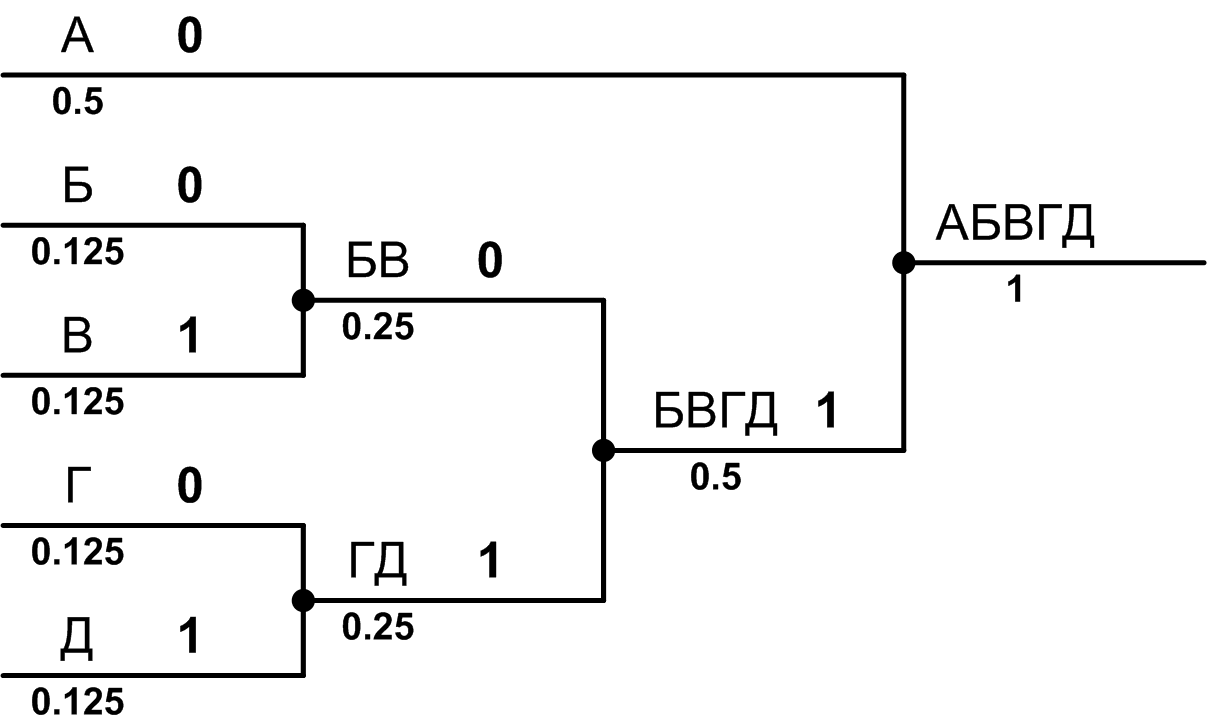
\includegraphics[height=0.2\textwidth]{pict/huffman}
        \caption{Алгоритм Хаффмана: кодирование}
        \label{pict:huffman}
    \end{center}
\end{figure} 
См. рисунок \ref{pict:huffman}
\end{verbatim}
\end{example}

\begin{example}[Форма]
\begin{figure}
    \begin{center}
        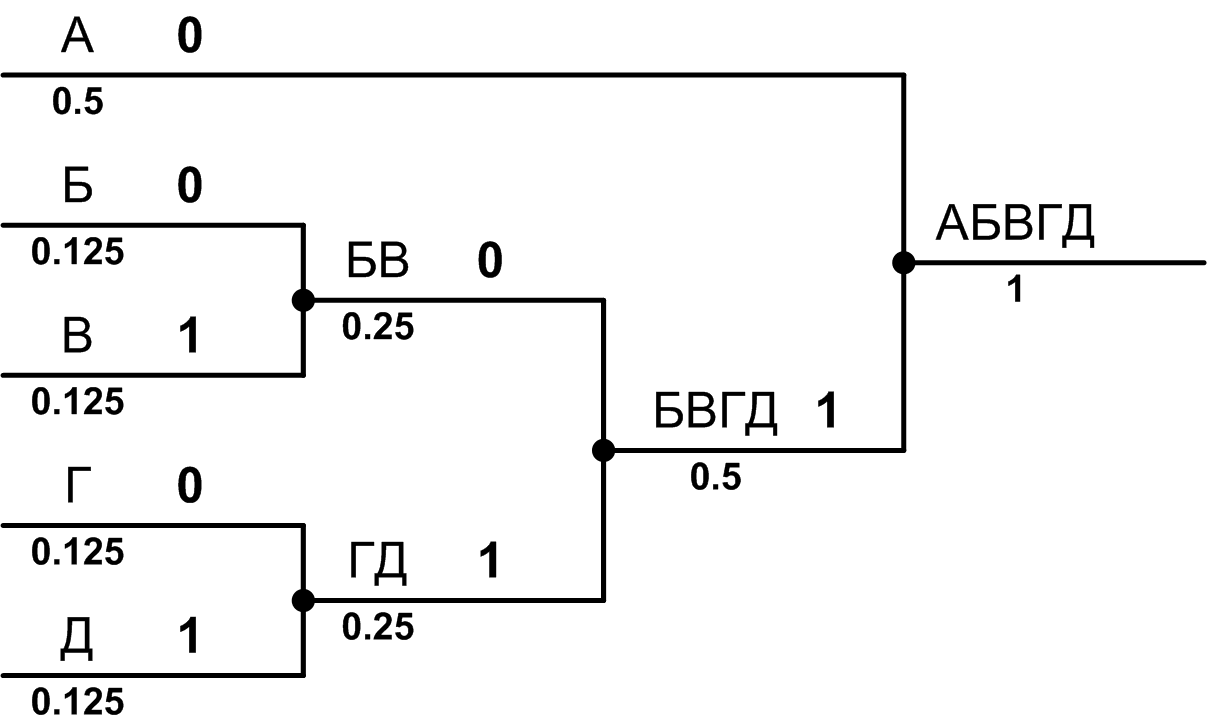
\includegraphics[height=0.2\textwidth]{pict/huffman}
        \caption{Алгоритм Хаффмана: кодирование}\label{pict:huffman}
    \end{center}
\end{figure} 
См. рисунок \ref{pict:huffman}
\end{example}
\end{frame}


\begin{frame}[fragile,allowframebreaks]
\frametitle{Ссылки на таблицы}
\begin{example}[Содержание]
\begin{verbatim}
\begin{table}[ht]   \caption{Пример таблицы}
                    \label{t:pifagor}
    \begin{tabular}[c]{|l|l|l|}
        \hline\hline
        $a$ & $b$ & \rotatebox{90}{$c=\sqrt{a^2+b^2}$}\\ 
        \hline\hline
        3   & 4   & 5          \\ \hline
        4   & 5   & $\sqrt{41}$\\ \hline
    \end{tabular}
\end{table}
См. таблицу \ref{t:pifagor}
\end{verbatim}
\end{example}

\begin{example}[Форма]
\begin{table}[ht]
\caption{Пример таблицы}\label{t:pifagor}
\centering
\begin{tabular}[c]{|l|l|l|}
\hline\hline
$a$ & $b$ & \rotatebox{90}{$c=\sqrt{a^2+b^2}$}\\ 
\hline\hline
3   & 4   & 5          \\ \hline
4   & 5   & $\sqrt{41}$\\ \hline
\end{tabular}
\end{table}
См. таблицу \ref{t:pifagor}
\end{example}
\end{frame}


\begin{frame}[fragile,allowframebreaks]
\frametitle{Ссылки}
\framesubtitle{Литература}
\begin{example}[Содержание]
\begin{verbatim}
Из книг по \LaTeXe\ можно рекомендовать 
\cite{bib:cotelnikov,bib:baldin}.
* * *
\begin{thebibliography}{99}
    \bibitem{bib:cotelnikov} Игорь Котельников,...
    \bibitem{bib:baldin} Балдин Е.М., Компьютерная,...
    * * *
\end{thebibliography}
\end{verbatim}
\end{example}

\begin{example}[Форма]
Из книг по \LaTeXe\ можно рекомендовать \cite{bib:cotelnikov,bib:baldin}.
\end{example}
\end{frame}

\begin{frame}[fragile,allowframebreaks]
    \frametitle{Ссылки на литературу правильно}
    \framesubtitle{bibtex}
    Заведём файл библиографии \verb"bibliobase.bib", содержащий записи о:
\begin{semiverbatim}  
%книгах:
@book\{bib:cotelnikov,
    author = \{И.Котельников and П.Чеботаев\},
    title = \{\{\\LaTeX\} по-русски\},
    publisher = \{Сибирский хронограф\},
    address = \{Новосибирск\},
    numpages = \{496\},
    language=\{russian\},
    year = \{2009\}
\}
\end{semiverbatim}  

\begin{semiverbatim}  
% статьях в журналах
@article\{kn:knuth:mf3,
    author = \{D. E. Knuth\},
    title = \{The New Versions of \{\\TeX\} and \{\\MF\}\},
    journal = \{TUGboat, the \{\\TeX\} User's Group Newsletter\},
    volume = 10,
    number = 3,
    pages = \{325--328\},
    month = \{nov\},
    year = 1989
\} 
\end{semiverbatim}  

\begin{semiverbatim}  
% интернет ссылках и прочем...
@misc\{bib:ctan,
    author = \{\},
    howpublished=\{\\url\{http://ctan.org/\}\},
    language=\{russian\},
    title = \{Comprehensive \{\\TeX\} Archive Network\}
\}
\end{semiverbatim}  

Теперь, чтобы возложить работу на плечи \verb"bibtex", следует вместо окружения \verb"thebibliography" использовать пару команд:
\begin{semiverbatim}  
\\bibliographystyle\{<имя стиля оформления библиографии>\}
\\bibliography\{<путь к файлу в формате bibtex>\}
\end{semiverbatim}  

\end{frame}


\appendix

\begin{frame}[allowframebreaks]{Библиография}
\begin{thebibliography}{99}
    \bibitem{bib:cotelnikov} Игорь Котельников, Платон Чеботаев, <<\LaTeX по-русски>>
    \bibitem{bib:baldin} Балдин Е.М., Компьютерная типография \LaTeX
    \bibitem{bib:knuthAllAbout} Дональд Э. Кнут, Все про \TeX
    \bibitem{bib:knuthTypograph} Дональд Э. Кнут, Компьютерная типография
\end{thebibliography}
\end{frame}


\end{document}
